\documentclass[11pt,a4paper]{article}
\usepackage{cite}
\usepackage{amsthm}
\usepackage{amsfonts}
\usepackage{amsmath}
\usepackage{graphicx}
\usepackage{tikz}
\usepackage{caption}
\usepackage{booktabs}
\usepackage{amssymb}
\usepackage{algorithm}
\usepackage[noend]{algpseudocode}
\usepackage{amsmath}
\usepackage{verbatim}
\usetikzlibrary{calc}
\algnewcommand\True{\textbf{true}}
\algnewcommand\False{\textbf{false}}
\usepackage{listings}             % Include the listings-package
\lstset{language=C}  
\usepackage{graphviz}
\usepackage{subcaption}
\usepackage{adjustbox}
\usepackage{tkz-euclide}

\usepackage{graphicx,epstopdf}
\epstopdfsetup{update}
\DeclareGraphicsExtensions{.ps}
\epstopdfDeclareGraphicsRule{.ps}{pdf}{.pdf}{ps2pdf -dEPSCrop -dNOSAFER #1 \OutputFile}


\newcommand{\pinspins}{pins2pins}
\newcommand{\mcrl}{mCRL2}
\newcommand{\promela}{Promela}
\newcommand{\prob}{prob}
\newcommand{\dve}{DVE}
\newcommand{\uppaal}{UPPAAL}
\newcommand{\ltsmin}{LTSmin}
\newcommand{\pins}{PINS}
\newcommand{\algorithmicbreak}{\textbf{break}}
\newcommand{\Break}{\State{\algorithmicbreak}}


\begin{document}

\newtheorem{mydef}{Definition}
\title{Symbolic Model Checking of Timed Automata using \ltsmin{}}
\author{Sybe van Hijum}
\date{\today{}}
\maketitle

\clearpage
\tableofcontents

\clearpage
\section{Introduction}
Timed automata~\cite{Alur1994183} is a widely used modelling formalism. A recent usage of this formalism is the modelling of biological signalling pathways~\cite{DBLP:conf/bibe/SchivoSWCVKLPP12}. ANIMO is a tool that generates these timed automata from biological signalling pathways models. This leads however to large state spaces, and sometimes to models that are too large to handle by conventional methods. Therefore better model checking techniques for timed automata, that can handle larger state spaces are needed. We look into symbolic algorithms for timed automata.

BDDs (Binary Decision Diagrams)~\cite{Akers:1978:BDD:1310167.1310815,1676819} and variations like LDDs (List Decision Diagrams)~\cite{so62465} and MDDs (Multi-valued Decision Diagrams)~\cite{129849} have proven their value in model checking algorithms. Due to advances in this field, models with much larger state spaces can be explored on the same machine. This progress has not been translated directly to more efficient methods for timed automata. Several methods have been proposed, like CDDs (Clock Difference Diagrams)~\cite{BRICS19491}, CMDs (Constraint Matrix Diagrams)~\cite{5702245}, CRDs (Clock Restriction Diagrams)~\cite{crds} and DDDs (Difference Decision Diagrams)~\cite{ddds, ddd-datastructure-99}. All of these methods show some extra difficulties or limitations over BDDs. Also after their introduction they have not been developed further.

LTSmin~\cite{eemcs18152,ltsmin-mc:nmf2011} is a language independent on the fly model checker with several algorithmic back-ends. Its symbolic back-end uses BDDs to both represent the state space and the transition relations of models. These BDDs are generated on the fly by the search algorithms. LTSmin has a language module for the UPPAAL~\cite{UPPAAL} through the Opaal~\cite{opaal} lattice model checker. Through this module UPPAAL models can be loaded into LTSmin. For this language currently, only the multi-core back-end can be used~\cite{eemcs21972}. This multi-core approach showed efficient enough to compete with the latest version of the UPPAAL model checker. It showed significant speedups on multi-core machines, at the cost of some memory increase however. To tackle the memory increase a combination of the Opaal front-end and the symbolic back-end could be a solution.

The symbolic back-end of LTSmin provides both a memory reduction by using BDDs and a speedup by using multi-threaded search algorithms and the multi-threaded BDD package Sylvan~\cite{sylvan}. Using this together with the UPPAAL language front-end will hopefully result in a model checker that can compete both on time and memory consumption with the UPPAAL model checker.

We will propose a symbolic reachability for timed automata that is capable of handling the models that are generated by the ANIMO tool.

%

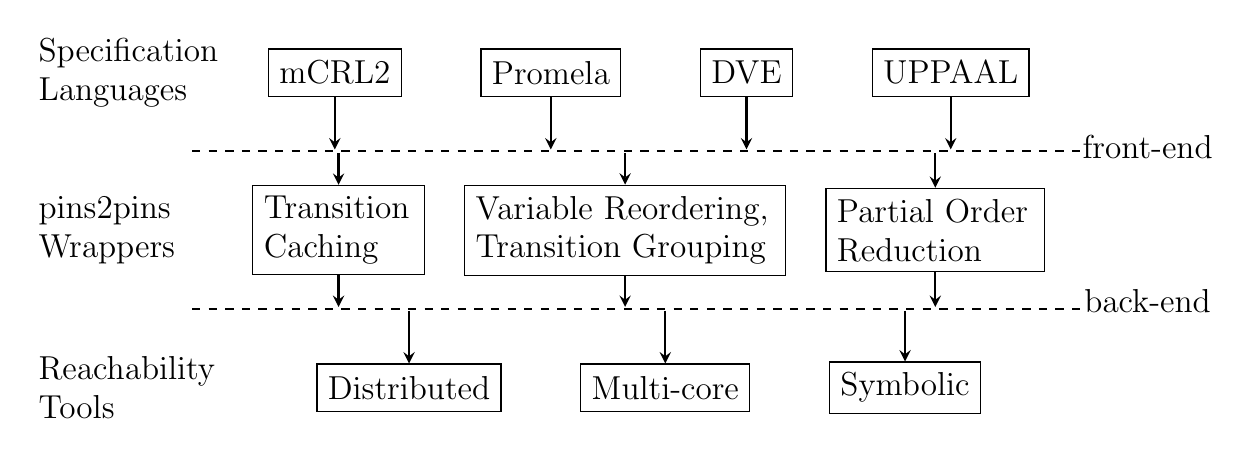
\begin{tikzpicture}[node distance=2cm]
	\large
    \begin{scope}[yshift=4cm]
        \node[node distance=2cm, text width=2.5cm] (speclan) {Specification Languages};
        \node[below of=speclan, node distance=2cm, text width=2.5cm] (p2p) {\pinspins\\ Wrappers};
        \node[below of=p2p, node distance=2cm, text width=2.5cm] (reach) {Reachability Tools};
    \end{scope}    
    
    \begin{scope}[yshift=4cm, xshift=6.5cm]
        \matrix[nodes={draw}, column sep=1cm]{
            \node[minimum size=6mm] (mcrl2) {\mcrl}; &
            \node[minimum size=6mm] (promela) {\promela}; &
            \node[minimum size=6mm] (other) {\dve}; &
            \node[minimum size=6mm] (prob) {\uppaal}; \\
        };
        \node[right of=prob, node distance=2.5cm] (placeholder) {};
        \node[below of=placeholder, node distance=0.95cm, inner sep=0cm] {front-end};
        \node[below of=placeholder, node distance=2.9cm, inner sep=0cm] {back-end};
        
        \node[below of=mcrl2, node distance=1cm, inner sep=0cm] (a) {};
        \node[below of=promela, node distance=1cm, inner sep=0cm] (b) {};
        \node[below of=other, node distance=1cm, inner sep=0cm] (c) {};
        \node[below of=prob, node distance=1cm, inner sep=0cm] (d) {};
        
        \draw (mcrl2) edge[thick, -stealth] (a);
        \draw (promela) edge[thick, -stealth] (b);
        \draw (other) edge[thick, -stealth] (c);
        \draw (prob) edge[thick, -stealth] (d);
    \end{scope}
    
    \draw[thick, dashed](.7,3cm)--(12,3cm);

    \begin{scope}[yshift=2cm, xshift=6.5cm]
        \matrix[nodes={draw}, column sep=.5cm]{
            \node[text width=1.9cm, minimum size=10mm] (cach) {Transition Caching}; &
            \node[text width=3.8cm, minimum size=10mm] (reord) {Variable Reordering, Transition Grouping}; &
            \node[text width=2.5cm, minimum size=10mm] (por) {Partial Order Reduction}; \\
        };
        \node[above of=cach, node distance=1cm, inner sep=0cm] (a) {};
        \node[above of=reord, node distance=1cm, inner sep=0cm] (b) {};
        \node[above of=por, node distance=1cm, inner sep=0cm] (c) {};
        
        \node[below of=cach, node distance=1cm, inner sep=0cm] (d) {};
        \node[below of=reord, node distance=1cm, inner sep=0cm] (e) {};
        \node[below of=por, node distance=1cm, inner sep=0cm] (f) {};
        
        \draw (a) edge[thick, -stealth] (cach);
        \draw (b) edge[thick, -stealth] (reord);
        \draw (c) edge[thick, -stealth] (por);
        
        \draw (cach) edge[thick, -stealth] (d);
        \draw (reord) edge[thick, -stealth] (e);
        \draw (por) edge[thick, -stealth] (f);
    \end{scope}
    
    \draw[thick, dashed](.7,1cm)--(12,1cm);
    
    \begin{scope}[xshift=6.5cm]
        \matrix[nodes={draw}, column sep=1cm]{
            \node[minimum size=6mm] (dist) {Distributed}; &
            \node[minimum size=6mm] (mult) {Multi-core}; &
            \node[minimum size=6mm] (sym) {Symbolic}; \\
        };
        
        \node[above of=dist, node distance=1cm, inner sep=0cm] (a) {};
        \node[above of=mult, node distance=1cm, inner sep=0cm] (b) {};
        \node[above of=sym, node distance=1cm, inner sep=0cm] (c) {};
        
        \draw (a) edge[thick, -stealth] (dist);
        \draw (b) edge[thick, -stealth] (mult);
        \draw (c) edge[thick, -stealth] (sym);
    \end{scope}    
    
\end{tikzpicture}

\clearpage
\section{Preliminaries}
We will first define timed automata and zones, a method used to represent time in timed automata. Also a subsumption check over zones will be defined. 

\subsection{Timed Automata}
Timed automata is a formalism that extends labelled transition systems with one or more clocks. Guards over these clocks, denoted as $G(C)$ can be used for transitions and as invariants. 

\begin{mydef}[Clock Guards]
\label{def:clockGuards}
$G(C)$ is the set of conjunctions over simple conditions of the form $x \Join c$ or $x-y \Join c$, where $x,y \in C$, $c \in \mathbb{N}$ and $\Join \in \{<,\leq,=,\geq,>\}$.
\end{mydef}

Timed automata use a notion of downwards closed clock invariants. We define a downwards closed set and specify this for clock guards.

\begin{mydef}[Downwards Closed Set]
A set $A$ is downwards closed if $\forall a \in A. x \preceq a \implies x \in A$. 
\end{mydef}

For clock guards we define the operator $\preceq$ to be true for $x \Join c \preceq x \Join' c'$ if $c < c'$ or $c = c'$ and $\Join = < \wedge \Join' = \leq$. This leads to a much simpler definition of downwards closed clock guards.

\begin{mydef}[Downwards Closed Clock Guards]
A set $G(C)$ is downwards closed if all simple conditions are of the form $x \Join c$ or $x-y \Join c$, where $x,y \in C$, $c \in \mathbb{N}$ and $\Join \in \{<,\leq\}$.
\end{mydef}


Also reset actions for clock can be defined for transitions, setting clocks to $0$. All clocks in the system will increase at the same rate. As our work continues on~\cite{eemcs21972} we use the same definition of timed automata.

\begin{mydef}[Timed Automata]
\label{def:TA}
An extended timed automaton is a 6-tuple A = $\langle L, C, Act, l_0, \rightarrow, I_c\rangle$ where
{\renewcommand\labelitemi{--}
	\begin{itemize}
		\item L is a finite set of locations, typically denoted by $l$
		\item C is a finite set of clocks, typically denoted by c
		\item Act is a finite set of actions
		\item $l_0 \in$ L is the initial location
		\item $\rightarrow \subseteq L \times G(C) \times Act \times 2^C \times L$ is the (non-deterministic) transition relation. We normally write l $\stackrel{g,a,r}{\longrightarrow}$ l' for a transition., where l is the source location, g is the guard over the clocks, a is the action, and r is the set of clocks reset.
		\item $I_C : L \rightarrow G(C)$ is a function mapping locations to downwards closed clock invariants.
	\end{itemize}
}
\end{mydef}

In the rest of this thesis we will not strictly stick to the definition of locations. We use the terminology 'locations' and other 'discrete variables'. Locations are the locations in the \uppaal{} transition system editor, the other discrete variables are declared in the C-like syntax that \uppaal{} uses. With the definition of a timed automaton we can combine a finite number of timed automata to a network of timed automata, which is a parallel composition, to define larger systems. This is a parallel composition that synchronizes on a set of channels $Chan$~\cite{UPPAAL}. $ch!$ and $ch?$ represent the output and input action on the channel $ch \in Chan$.

\begin{mydef}[Network of timed automata~\cite{eemcs21972}]
\label{def:networkTA}
Let Act = $\{ch!,ch?|ch \in Chan\} \cup \{\tau\}$ be a finite set of actions, and let C be a finite set of clocks. Then the parallel composition of extended timed automata $A_i = \langle L_i, C, Act, l^i_0, \rightarrow_{i}, I^i_C\rangle$ for all $1 \leq i \leq n$, where $n \in \mathbb{N}$, is a network of timed automata, denoted $A = A_1||A_2||..||A_n$.
\end{mydef}

\subsection{Zones}
For basic transition systems the state space can grow exponentially for the number of variables in the system. The state space of timed automata is by definition infinite, as clocks have real values. If a discrete state is defined between two points in time, an infinite amount of moments in time can happen during that state. Even when some granularity is used, that defines that clocks will only increase with certain step size the automata can still have infinite state space if a clock is unbounded. To tackle this problem most model checkers use a notion of zones for the representation of time. A zone can be seen as a set of clock guards. To represent these zones several data structures have been developed. One of the most common used structures are Difference Bound Matrices (DBMs)~\cite{dbmorig,bengtsson2002clocks}.

\begin{mydef}[Difference Bound Matrix]
A DBM for the clocks $C = \{c_1,...c_n\}$ is a $(n+1)^2$ matrix. Each position has the following attributes.

\begin{tabular}{lll}
Attribute                & Type                      & Description                                           \\\hline
const(i,j)               & $\mathbb{Z}$             & Constant value $c$ \\
op(v)                    & \{$<$, $\leq\}$     & Operator $<$ or $\leq$.                         \\
\end{tabular}

Each position $(i,j)$ defines an upper bound on the value of $c_i - c_j$. On the first row and first column an extra clock $\mathbf{O}$ is added as $c_0$ with constant value 0. 
\end{mydef}
 
These matrices use both a column and a row for each clock, and on each position $(i,j)$ an upper bound on the difference between the clocks $c_i$ and $c_j$ is given in the form $c_i - c_j \preceq x$ where $\preceq \in \{<, \leq\}$ and $x \in \mathbb{Z}$. For the constraints over the single clocks an extra clock $\mathbf{O}$ with a constant value 0 is added. This way the upper and lower bound of a clock $c_i$ can be given by $c_i - \mathbf{O} \preceq x$ and $\mathbf{O} - c_i \preceq y$. The addition of this $\mathbf{O}$ clock will give the matrix of a timed automaton always size $(|C|+1)^2$. This way convex zones of clock variables can be represented. Each matrix can however only contain a single convex zone. Concave zones and multiple convex zones need multiple matrices to be represented. As a solution often a list of DBMs is used. In figure \ref{fig:dbm} we give an example of a DBM with two clocks: $c_1$ and $c_2$, representing the zone $0 \leq c_1 < 5 \wedge 0 \leq c_2 \leq 4$. The diagonal only contains $(0,\leq)$ values as these elements give the difference between a clock and itself, which is clearly always 0.

\begin{figure}
	\centering
	\begin{math}
% 		\begin{pmatrix}
 \bordermatrix{ 		                 & \mathbf{O} & c_1           & c_2        \cr
 			\mathbf{O} &(0,\leq)      & (0,\leq)      & (0,\leq)     \cr
 			c_1        &(5,<   )      & (0,\leq)      & (\infty,\leq)\cr
 			c_2        &(4,\leq)      & (\infty,\leq) & (0,\leq)     \cr}
% 		\end{pmatrix}
	\end{math}
	\caption{DBM}
	\label{fig:dbm}
\end{figure}

A number of operations on DBMs has been defined. We will introduce the operations we use. The same notation as~\cite{eemcs21972} is used.
\begin{itemize}
\item $D \uparrow$ is called the delay operator. This lets time pass unlimitedly from the zone in D.
\item $D \cap D'$ adds additional constraints from $D'$ to $D$. This is used for transitions that have clock constraints. These constraints can be represented as a DBM.
\item $D[r]$ with $r \subseteq C$, resets all clocks in $r$.
\item $D/B$ does a maximal bounds extrapolation. In section \ref{subsec:extrapolation} we will go into more detail about this extrapolation.

\end{itemize}

\subsection{Zone subsumption}
\label{subsec:subsumtion}
In model checking an important function is to check if a certain state has been visited already earlier. For normal automata this can be done by comparing the newly found state to all states that have already been visited, and check if one of those states is equal to that new state. This is often done by more efficient methods, like hash functions, but the equality check remains. For states with zones this equality check does not suffice. Two zones do not need to be equal, but the newly discovered zone can also be a subset of the earlier discovered zones. In \ltsmin{} this is done by a subsumption check~\cite{eemcs21972} that is performed over the DBMs. This check is delegated to the \uppaal{} DBM library. The function checks if a new zone is a subset of the zone represented by a DBM.

\subsection{Binary Decision Diagram}
We shortly introduce binary decision diagrams(BDDs)~\cite{Bryant:1986:GAB:6432.6433}. BDDs are the basis of most symbolic model checking techniques. BDDs are a way to represent boolean functions. All diagrams that we discuss in the rest of this thesis are based on BDDs.
\begin{figure}[h]
\centering
	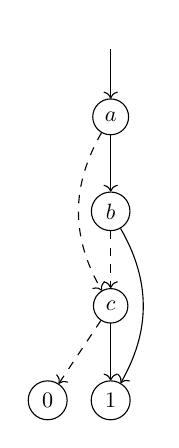
\begin{tikzpicture}[
		smallvertex/.style={circle,draw,scale=0.8}
		]
		\node[smallvertex](S1){$a$};
		\node[smallvertex, draw = none, above of = S1, yshift = 0.25cm](S0){};
		
		\node[smallvertex, below of = S1, yshift = -.5cm](S2){$b$};
		\node[smallvertex, below of = S2, yshift = -.5cm](S3){$c$};
		\node[smallvertex, below of = S3, yshift = -.5cm](S4){$1$};
		\node[smallvertex, left of = S4](S5){$0$};
		
		\draw[->] (S0) --(S1) node [midway, above, sloped, scale=0.75,
		rotate=0, xshift =-0.4 cm, yshift = -0.2cm]{};
		\draw[->] (S1) --(S2) node [midway, above, sloped, scale=0.75,
		rotate=90, xshift =-0.4 cm, yshift = -0.2cm]{};
		\draw[dashed,->] (S2) --(S3) node [midway, above, sloped, scale=0.75,
		rotate=90, xshift =-0.4 cm, yshift = -0.2cm]{};
		\draw[->] (S3) --(S4) node [midway, above, sloped, scale=0.75,
		rotate=90, xshift =-0.4 cm, yshift = -0.2cm]{};		
		\draw[->,dashed] (S1) edge[bend right](S3) node [midway, above, sloped, scale=0.75,
		rotate=90, xshift =-0.4 cm, yshift = -0.2cm]{};	
		\draw[->] (S2) edge[bend left](S4) node [midway, above, sloped, scale=0.75,
		rotate=90, xshift =-0.4 cm, yshift = -0.2cm]{};	
		\draw[dashed,->] (S3) --(S5) node [midway, above, sloped, scale=0.75,
		rotate=90, xshift =-0.4 cm, yshift = -0.2cm]{};
		[bend left]
	\end{tikzpicture}
\caption{A BDD representing $(a \wedge b) \vee c$}
\label{fig:BDD}
\end{figure}



\begin{mydef}[Binary Decision Diagram~\cite{Bryant:1986:GAB:6432.6433}]
A BDD is a rooted, directed graph with vertex set $V$ containing two types of vertices. A nonterminal vertex $v$ has as attributes an argument index $index(v) \in \{1,...,n\}$, and two children $low(v),high(v) \in V$. A terminal vertex $v$ has as attribute a value $value(v) \in \{0,1\}$
\end{mydef}



\begin{mydef}[BDD Semantics~\cite{Bryant:1986:GAB:6432.6433}]
A BDD $G$ having root vertex $v$ denotes a function $f_v$ defined recursively as:
\begin{itemize}
\item If $v$ is a terminal vertex:
\begin{itemize}
\item If $value(v)=1$, then $f_v=1$
\item If $value(v)=0$, then $f_v=0$
\end{itemize}
\item If $v$ is a nonterminal vertex with $index(v)=i$ then $f_v$ is the function
$f_v(x_1,...,x_n) = \overline{x_i}\cdot f_{low(v)}(x_1,...,x_n)+x_i\cdot f_{high(v)}(x_1,...,x_n)$.
\end{itemize}
\end{mydef}

The high and low edges of a node are graphically shown as a straight and a dotted line respectively. A BDD can also be reduced and ordered, we will not go into detail on that here. In Figure \ref{fig:BDD} we show a BDD representing the boolean formula $(a \wedge b) \vee c$. For larger diagrams, edges that go directly to the terminal vertex with value $0$ are often omitted for better readability. 

\clearpage
\section{Related Work}
In this related work section we will discuss a number of methods used for model checking timed automata. We will choose a method to extend our work on, and go more into detail on that method.

\subsection{Methods}
Already several model checkers for timed automata exist such as \uppaal{}~\cite{UPPAAL}, KRONOS~\cite{kronos}, RABBIT~\cite{CAV03} and RED~\cite{crds}. We focus mainly on the \uppaal{} tool as we use the same input format. Opaal~\cite{opaal}, the language module for \ltsmin{}, uses the XML format that is created by the \uppaal{} tools. This way we can use the \uppaal{} user interface to create and adapt models. We also use the \uppaal{} DBM library to represent zones. Several methods exist to represent the clock variables in a timed model. The most used methods are digitization and zones. 

Digitization approximates the continuous values of clocks by using discrete values~\cite{CHARME01}. The method however only works for closed timed automata, meaning that no strict comparisons on clocks can be made in the model and that clocks only can be compared to integers. This approach is very sensitive to the granularity of the values used and the upper bound of the clock values. When fine granularity or large upper bounds are used, the memory usage will increase too much. An advantage of this approach is that basic model checking approaches can be used and no extra complexity due to zone calculations is added. This method results in a transition system with only discrete variables, so a normal BDD package can be used. In ~\cite{nguyen2012discrete} a similar approach is proposed by using clock tick actions to represent time progress and removing clock variables altogether. 

The most established method to represent clock zones are DBMs. We gave an introduction to this structure in the preliminaries section. Several methods based on BDDs have been developed to represent zones. All of these are similar to DBMs in the sense that they use clock constraints to represent the zones. These structures use a BDD-like structure to represent the zones more efficiently. Below we shortly describe four methods. For each method we give an example, all examples represent $2 < c_1 - c_2 < 4 \vee 7 \leq c_1 - c_2 \leq 8$.

CDDs~\cite{BRICS19491} use single nodes for each variable and have multiple disjoint intervals for that variable on the edges. This results in a node with a larger fanout. The upper and lower bound for each pear of clocks are represented in a single node, as the edges represent intervals. Requiring the disjointness of intervals can lead to a memory inefficient representation, as intervals need to be cut in more smaller parts. All algorithms on CDDs do not maintain disjointness, after every step it needs to be re-established. In figure \ref{fig:cdd-example} we have an example of a CDD.

\begin{figure}[h]
\begin{center}
	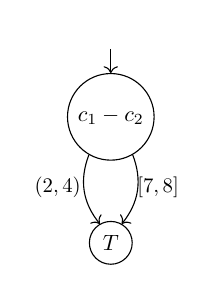
\begin{tikzpicture}[
		smallvertex/.style={circle,draw,scale=0.8}
		]
			
		\node[smallvertex](S0){$c_1 - c_2$};
	    \node[smallvertex, draw = none, above of = S0, yshift = 0.25cm](S4){};
		\draw[->] (S4) --(S0) node [midway, above, sloped, scale=0.75,
		rotate=295, xshift =-0.4 cm, yshift = -0.2cm]{};
		\node[smallvertex, below of = S0, yshift = -1cm](S3){$T$};
		\draw[->] (S0) edge [bend left](S3) node [midway, above, sloped, scale=0.75,
		rotate=0, xshift =-0.9 cm, yshift = -1.5cm]{$(2,4)$};
		\draw[->] (S0) edge [bend right](S3) node [midway, above, sloped, scale=0.75,
		rotate=0, xshift =0.8 cm, yshift = -1.5cm]{$[7,8]$};
	\end{tikzpicture}
\end{center}
\caption{CDD representation}
\label{fig:cdd-example}
\end{figure}

DDDs~\cite{ddds, ddd-datastructure-99} use a upper-bound constraint on each node that can either be true or false. Each node thus has a fixed fanout of two. When a constraint is false, a next node will have another constraint on the same variable. This requires a fixed ordering based on the variables, values and operators. In figure \ref{fig:ddd-example} an example of a DDD is shown.

\begin{figure}[h]
\begin{center}
	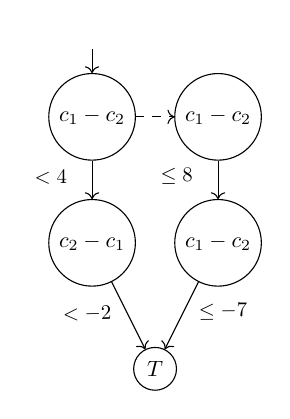
\begin{tikzpicture}[
		smallvertex/.style={circle,draw,scale=0.8}
		]
			
		\node[smallvertex](S0){$c_1 - c_2$};
		\node[smallvertex, draw = none, above of = S0, yshift = 0.25cm](S5){};
		\draw[->] (S5) --(S0) node [midway, above, sloped, scale=0.75,
		rotate=295, xshift =-0.4 cm, yshift = -0.2cm]{};
		\node[smallvertex, right of = S0, xshift = 1cm](S1){$c_1 - c_2$};
		\draw[dashed,->] (S0) --(S1) node [midway, above, sloped, scale=0.75,
		rotate=0, xshift =-0.7 cm, yshift = -0.2cm]{};
		\node[smallvertex, below of = S0, yshift = -1cm](S2){$c_2 - c_1$};
		\draw[->] (S0) --(S2) node [midway, above, sloped, scale=0.75,
		rotate=90, xshift =-0.7 cm, yshift = -0.2cm]{$< 4$};
		\node[smallvertex, below of = S1, yshift = -1cm](S3){$c_1 - c_2$};
		\draw[->] (S1) --(S3) node [midway, above, sloped, scale=0.75,
		rotate=90, xshift =-0.7 cm, yshift = -0.2cm]{$\leq 8$};
		\node[smallvertex, below of = S0, xshift = 1cm, yshift = -3cm](S4){$T$};
		\draw[->] (S2) --(S4) node [midway, above, sloped, scale=0.75,
		rotate=65, xshift =-0.7 cm, yshift = -0.2cm]{$<-2$};
		\draw[->] (S3) --(S4) node [midway, above, sloped, scale=0.75,
		rotate=297, xshift =0.7 cm, yshift = -0.2cm]{$\leq-7$};
	\end{tikzpicture}
\end{center}
\caption{DDD representation}
\label{fig:ddd-example}
\end{figure}

CRDs~\cite{crds} differ mainly from CDDs by not using disjoint intervals but possibly overlapping upper bounds, for a pair of variables on their edges. This diagram will have a larger fanout per node, like CDDs. Several normal forms for this diagram are proposed, with different performance results. It is also shown that CRDs can be combined with BDDs into a single structure to fully symbolic represent state space. In figure \ref{fig:crd-example} we give an example of a CRD.

\begin{figure}[h]
\begin{center}
	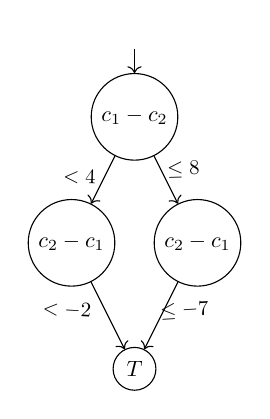
\begin{tikzpicture}[
		smallvertex/.style={circle,draw,scale=0.8}
		]
		\node[smallvertex](S0){$c_1 - c_2$};
		\node[smallvertex, draw = none, above of = S0, yshift = 0.25cm](S4){};
		\draw[->] (S4) --(S0) node [midway, above, sloped, scale=0.75,
		rotate=295, xshift =-0.4 cm, yshift = -0.2cm]{};
		\node[smallvertex, below of = S0, yshift = -1 cm, xshift = -1 cm](S1){$c_2 - c_1$};
		\node[smallvertex, below of = S0, yshift = -1 cm, xshift = 1  cm](S2){$c_2 - c_1$};
		\draw[->] (S0) --(S1) node [midway, above, sloped, scale=0.75,
		rotate=295, xshift =-0.4 cm, yshift = -0.2cm]{$<4$};
		\draw[->] (S0) --(S2) node [midway, above, sloped, scale=0.75,
		rotate=65, xshift =0.3 cm, yshift = -0.1cm]{$\leq 8$};
		\node[smallvertex, below of = S0, yshift = -3cm](S3){$T$};
		\draw[->] (S1) --(S3) node [midway, above, sloped, scale=0.75,
		rotate=60, xshift =-0.7 cm, yshift = -0.2cm]{$<-2$};
		\draw[->] (S2) --(S3) node [midway, above, sloped, scale=0.75,
		rotate=300, xshift =0.4 cm, yshift = -0.2cm]{$\leq-7$};
	\end{tikzpicture}
\end{center}
\caption{CRD representation}
\label{fig:crd-example}
\end{figure}

CMDs~\cite{5702245} combine CDDs, CRDs and DBMs into a single structure. This diagram type differs from the others by having multiple constraints per edge, resulting in a diagram with few nodes. Upper- and lower-bounds of multiple clock pairs can be on a single edge. CMDs do not have a canonical form so only some reductions are proposed. An example of a CMD is given in figure \ref{fig:cmd-example}. This figure contains two examples, the first is a diagram of the constraint we use in this section. To show the difference with other diagrams we also give a diagram representing the same zone as the DBM in figure \ref{fig:dbm}.

\begin{figure}[h]
%\begin{center}
\begin{subfigure}{.5\textwidth}
	\begin{tikzpicture}[
		smallvertex/.style={circle,draw,scale=0.8}
		]
			
		\node[smallvertex](S0){ };
		\node[smallvertex, draw = none, above of = S0, yshift = 0.25cm](S4){};
		\draw[->] (S4) --(S0) node [midway, above, sloped, scale=0.75,
		rotate=295, xshift =-0.4 cm, yshift = -0.2cm]{};
		\node[smallvertex, below of = S0, yshift = -1cm](S3){$T$};
		\draw[->] (S0) edge [bend left](S3) node [midway, above, sloped, scale=0.75,
		rotate=0, xshift =-1.5 cm, yshift = -1.5cm]{$2<c_1-c_2<4$};
		\draw[->] (S0) edge [bend right](S3) node [midway, above, sloped, scale=0.75,
		rotate=0, xshift =1.5 cm, yshift = -1.5cm]{$7\leq c_1-c_2\leq8$};
	\end{tikzpicture}	
\end{subfigure}	
\begin{subfigure}{.5\textwidth}
	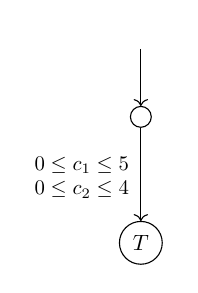
\begin{tikzpicture}[
		smallvertex/.style={circle,draw,scale=0.8}
		]
			
		\node[smallvertex](S0){ };
		\node[smallvertex, draw = none, above of = S0, yshift = 0.25cm](S4){};
		\draw[->] (S4) --(S0) node [midway, above, sloped, scale=0.75,
		rotate=295, xshift =-0.4 cm, yshift = -0.2cm]{};
		\node[smallvertex, below of = S0, yshift = -1cm](S3){$T$};
		\draw[->] (S0) edge (S3) node [midway, above, sloped, scale=0.75,		
		rotate=0, xshift =-1 cm, yshift = -1.5cm, align=center]{$0 \leq c_1 \leq 5$\\$ 0 \leq c_2 \leq 4$};
	\end{tikzpicture}
\end{subfigure}
%\end{center}
\caption{CMD representation}
\label{fig:cmd-example}
\end{figure}

In ~\cite{7098276, 7184781} a method is proposed purely based on BDDs by translating the constraints directly into BDD nodes. We call this method BDD zones. This results in a unified structure for both the discrete variables and the clock constraints. The method is only a proof of concept and has not been implemented in a model checker and no performance results are known. Subsumption for this method may be difficult. On BDDs only equalities can be checked, and no inequalities. This way inclusion is not trivial to check by normal BDD algorithms.

\begin{table}[]
\centering
\caption{Comparing Diagrams}
\label{table:diagrams}
\begin{tabular}{|l|l|l|}
\hline
Type                                                   & Pro                                                                                                                                                                                                                             & Con                                                                                                                                                                                                                                                          \\ \hline
DBM                                                    & \begin{tabular}[c]{@{}l@{}}Canonical form for convex zones\\ Existing library\\ Inclusion check\end{tabular}                                                                                                                    & \begin{tabular}[c]{@{}l@{}}Concave zones need multiple DBMs\\ Not memory efficient\end{tabular}                                                                                                                                                              \\ \hline
DDD                                                    & \begin{tabular}[c]{@{}l@{}}Structure like LDD\\ Re-ordering of variables possible\\ Apply same efficiency as BDDs\\ Boolean variables also in DDD\end{tabular}                                                                  & \begin{tabular}[c]{@{}l@{}}Canonicity hard to obtain\\ No on the fly canonicity\\ Expensive normal form computation\\ Only time performance tested\\ Only reduction algorithms\end{tabular}                                                                  \\ \hline
CDD                                                    & \begin{tabular}[c]{@{}l@{}}Structure like MDD\\ Inclusion check\\ (intersection of complement)\end{tabular}                                                                                                                     & \begin{tabular}[c]{@{}l@{}}No algorithm to get normal form\\ Only high level algorithms given\\ Methods don't maintain disjointness\\ Expensive normal form computation\\ No implementation results available\\ Disjointness memory inefficient\end{tabular} \\ \hline
CRD                                                    & \begin{tabular}[c]{@{}l@{}}Combination with BDD possible\\ Variable reordering shows advantage\\ Library available\\ Some benchmarks exp better than CDD\\ Extensive benchmarks\\ Good performance backwards reach\end{tabular} & \begin{tabular}[c]{@{}l@{}}3 possible canonical forms\\ No algorithms in paper\\ Some benchmarks linear worse than CDD\end{tabular}                                                                                                                          \\ \hline
CMD                                                    & Benchmarks against RED and \uppaal{} & \begin{tabular}[c]{@{}l@{}}Results differ per case\\ Needs translation from vector to edges\\ Two reduced forms\end{tabular}                                                                                                                                 \\ \hline
\begin{tabular}[c]{@{}l@{}}BDD\\ discrete\end{tabular} & \begin{tabular}[c]{@{}l@{}}Using existing BDD packages\\ Good performance for small clock values\end{tabular}                                                                                                                   & \begin{tabular}[c]{@{}l@{}}Performance decreases fast for large values\\ Not possible with current Opaal \pins{}\\ Introducing additional 'tick' actions\\ Only for closed timed automata\end{tabular}                                                          \\ \hline
\begin{tabular}[c]{@{}l@{}}BDD\\ zones\end{tabular}    & \begin{tabular}[c]{@{}l@{}}Using existing BDD packages\\ All variable reorderings possible\\ Only need direct translation DBM to\\ state vector\\ Easy to implement\end{tabular}                                                & \begin{tabular}[c]{@{}l@{}}Losing zone containment\\ No implementation results\end{tabular}                                                                                                                                                                  \\ \hline
\end{tabular}
\end{table}

A known difficulty in BDDs is the variable ordering. A bad ordering can lead to a BDD of exponential size, where a good ordering can sometimes lead to a significantly smaller diagram. Of the zone diagrams named above, only for CRDs experiments with different orderings have been conducted, the other researches assume a given ordering on the variables and the ordering of the values is fixed. The CRD case shows that full interleaving and having related variables close to each other in the ordering is preferable and gives the best results, both on speed and memory. This is the same result as expected with BDDs, this suggests that similar orderings should be used with these techniques. In Table \ref{table:diagrams} we compare the different types of diagrams we discussed above.

\begin{figure}[h] 
\input{pins}
\caption{Modular structure of \ltsmin{}}
\label{fig:pins_modern}
\end{figure}

\subsection{LTSmin}
\ltsmin{}~\cite{eemcs18152,ltsmin-mc:nmf2011} is a language independent model checker. It is built in a modular way such that new languages can be added by a \pins{} (Partitioned Next-State Interface) interface without too much effort, and new algorithms can be added easily. \ltsmin{} offers four different algorithmic back-ends for model analysis: symbolic, multi-core, sequential and distributed. All of these back-ends support different types of reduction and model checking. Several language modules have already been built for \ltsmin{} such as \mcrl{}, \promela{}, \dve{} and \uppaal{}. The modular structure of \ltsmin{} is shown in Figure \ref{fig:pins_modern}. The \pins{} is the core of \ltsmin{}. This interface abstracts as much as possible from the model without losing the structure. It represents states as fixed length integer arrays. The main function of the interface is a (partitioned) next-state function which returns the successor states. With these functions a state space can be generated on the fly. With the use of dependency matrices event locality can be determined statically~\cite{rwcmatrices}. With these matrices, more efficient symbolic algorithms can be used, the number of next-state calls can be reduced, efficient variable re-orderings can be used, and transition caching can be used. In the current \uppaal{} \pins{} the next-state function is not partitioned and therefore no meaningful dependency matrix is created, and none of these algorithms can be used. Also the DBM variable is only represented by a pointer, which is not a meaningful value for the transition system. \ltsmin{} uses the pointer to a DBM to do the subsumption check as described in section \ref{subsec:subsumtion}.

\subsection{Difference Decision Diagrams}

We have discussed several symbolic approaches for representing zones. All of these approaches have benefits and downsides over each other. We chose to develop one of these approaches in \ltsmin{}. We wanted a diagram that can store both discrete states and zones, this can either be done in the diagram, or in a combination of the diagram and BDD or LDD nodes. Also a subsumption check on the diagram should be possible. We chose from the four zone representing diagrams discussed earlier. The CDD approach was not chosen due to the memory inefficient disjoint intervals and their algorithms not maintaining these disjointness. The CMD approach is too similar to DBMs, on which we already have an approach. The choice between CRD and DDD was between two quite similar diagrams. We have decided to continue on the DDD. It is a diagram form that is closely related to LDDs, for which we already have a library, so we can reuse parts of the LDD library, and it is also quite compatible to the current \pins{} structure and its next-state function. The method still has some loose ends that need research, mostly on the algorithms and efficiently creating a canonical form. No results on the memory usage are available, which is normally the greatest benefit of a symbolic approach, so also on the results side we can extend the current research. 

So DDDs are a diagram type that seems to fit well in the current structure we have, but there is still room for some more research. First we give the definition of a DDD.

\begin{mydef}[Difference Decision Diagram~\cite{ddds}]
\label{def:DDD}
A difference decision diagram (DDD) is a directed acyclic graph $(V,E)$. The vertex set $V$ contains two terminals $0$ and $1$ with out-degree zero, and a set of non-terminal vertices with out-degree two and the following attributes.
\\\\
\begin{tabular}{lll}
Attribute                & Type                      & Description                                           \\\hline
pos(v), neg(v)           & \textbf{Var}              & Positive variable $x_i$, and negative variable $x_j$. \\
op(v)                    & \{\textless, $\leq\}$     & Operator \textless or $\leq$.                         \\
const(v)                 & $\mathbb{D}$              & Constant c.                                           \\
high(v), low(v)          & $V$                       & High-branch h, and low-branch l.                   
\end{tabular}
\captionof*{table}{}  
The set E contains the edges $(v,low(v))$ and $(v, high(v))$, where $v \in V$ is a non-terminal vertex.
\end{mydef}

Now we have the definition of the structure. We also give the semantics of this structure. 

\begin{mydef}[DDD semantics]
\label{def:Semantics1}
The semantics of a vertex is defined recursively by the function $\mathcal{V}: V \rightarrow \textbf{Exp}:$
\begin{itemize}
\item $\mathcal{V}[[0]] \myeq$ false,
\item $\mathcal{V}[[1]] \myeq$ true,
\item \begin{math} \mathcal{V}[[v]] \myeq
\begin{cases}
(pos(v) - neg(v) < const(v)) \rightarrow \mathcal{V}[[high(v)]],\mathcal{V}[[low(v)]]\text{if }op(v) = '<'\\
(pos(v) - neg(v) \leq const(v)) \rightarrow \mathcal{V}[[high(v)]],\mathcal{V}[[low(v)]]\text{if }op(v) = '\leq'
\end{cases}
\end{math}
\end{itemize}
\end{mydef}

In the semantics we only take the information on the high edges. The implicit information on the low edge is not used. A node can thus only represent an upper-bound which is either true or false, it can not implicitly represent a lower-bound on the same variable pair. This representation also makes it easier to work with the state-vectors of \ltsmin{}.

In ~\cite{ddds} a canonical form for DDDs is discussed, also called a fully reduced DDD. Only definitions are given here, no algorithms to reach this form. It is stated that it is difficult to reach this fully reduced form. It is not clear if they managed to make their apply function in such a way that it maintains canonicity, as the function for BDDs does. To reach canonicity, local reductions and ordering are a first step, but it is not enough due to dependencies among the constraints. For BDDs the local reductions and ordering are sufficient to reach a canonical form. First we give some notational shorthands and then we define an ordering and local reductions on DDDs.
%
\begin{center}
\begin{tabular}{lll}
$var(v)$   & $=$ & $(pos(v),neg(v))$   \\
$bound(v)$ & $=$ & $(const(v),op(v))$  \\
$cstr(v)$  & $=$ & $(var(v),bound(v))$
\end{tabular}
\end{center}

To order DDD nodes we use the operator $\prec$. This orders variables and variable pairs in a predefined order. It orders bounds by increasing constants, and the $\le$ operator before the $\leq$ operator. So a node $v$ with $bound(v) = (0,<)$ comes before $bound(u) = (0,\leq)$ which comes before $bound(w) = (1,<)$.

\begin{mydef}[Ordered DDD~\cite{ddds}]
\label{def:ODDD}
An ordered DDD (ODDD) is a DDD where each non-terminal vertex $v$ satisfies:
\begin{enumerate}
  \item $neg(v) \prec pos(v)$,
  \item $var(v) \prec var(high(v))$,
  \item $var(v) \prec var(low(v))$ or \\ $var(v) = var(low(v))$ and $bound(v) \prec bound(low(v))$.
\end{enumerate}
\end{mydef}

After ordering a DDD some local reductions can be defined to reduce the size of a DDD.

\begin{mydef}[Locally Reduced DDD~\cite{ddds}]
\label{def:RLDDD}
A locally reduced DDD ($R_LDDD$) is an ODDD satisfying, for all non-terminals u and v:
\begin{enumerate}
  \item $\mathbb{D} = \mathbb{Z}$ implies $\forall v. op(v) = '\leq'$,
  \item $(cstr(u),high(u),low(u)) = (cstr(v),high(v),low(v))$ implies $u = v$,
  \item $low(v) \neq high(v)$,
  \item $var(v) = var(low(v))$ implies $high(v) \neq high(low(v))$.
\end{enumerate}
\end{mydef}

We give an example of the last point in figure \ref{fig:rlddd}. Here both diagrams represent the same zone: $2 < c_1 - c_2 \leq 8$. The node with $< 4$ on the high edge is redundant in this example and can thus be removed. 

\begin{figure}[h]
\begin{center}
	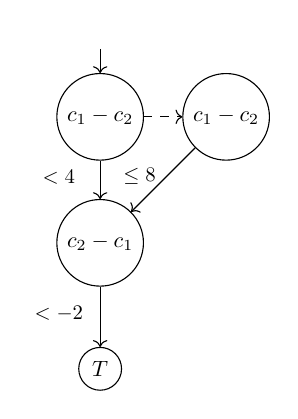
\begin{tikzpicture}[
		smallvertex/.style={circle,draw,scale=0.8}
		]
			
		\node[smallvertex](S0){$c_1 - c_2$};
		\node[smallvertex, draw = none, above of = S0, yshift = 0.25cm](S5){};
		\draw[->] (S5) --(S0) node [midway, above, sloped, scale=0.75,
		rotate=295, xshift =-0.4 cm, yshift = -0.2cm]{};
		\node[smallvertex, right of = S0, xshift = 1cm](S1){$c_1 - c_2$};
		\draw[dashed,->] (S0) --(S1) node [midway, above, sloped, scale=0.75,
		rotate=0, xshift =-0.7 cm, yshift = -0.2cm]{};
		\node[smallvertex, below of = S0, yshift = -1cm](S2){$c_2 - c_1$};
		\draw[->] (S0) --(S2) node [midway, above, sloped, scale=0.75,
		rotate=90, xshift =-0.7 cm, yshift = -0.2cm]{$< 4$};
		\draw[->] (S1) --(S2) node [midway, above, sloped, scale=0.75,
		rotate=315, xshift =-0.4 cm, yshift = -0.2cm]{$\leq 8$};
		\node[smallvertex, below of = S0, yshift = -3cm](S4){$T$};
		\draw[->] (S2) --(S4) node [midway, above, sloped, scale=0.75,
		rotate=90, xshift =-0.7 cm, yshift = -0.2cm]{$<-2$};
	\end{tikzpicture}
	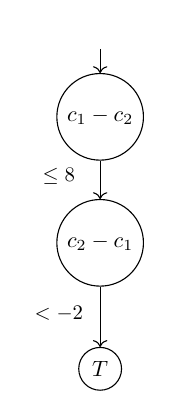
\begin{tikzpicture}[
		smallvertex/.style={circle,draw,scale=0.8}
		]
			
		\node[smallvertex](S0){$c_1 - c_2$};
		\node[smallvertex, draw = none, above of = S0, yshift = 0.25cm](S5){};
		\draw[->] (S5) --(S0) node [midway, above, sloped, scale=0.75,
		rotate=295, xshift =-0.4 cm, yshift = -0.2cm]{};
		\node[smallvertex, below of = S0, yshift = -1cm](S2){$c_2 - c_1$};
		\draw[->] (S0) --(S2) node [midway, above, sloped, scale=0.75,
		rotate=90, xshift =-0.7 cm, yshift = -0.2cm]{$\leq 8$};
		\node[smallvertex, below of = S0, yshift = -3cm](S4){$T$};
		\draw[->] (S2) --(S4) node [midway, above, sloped, scale=0.75,
		rotate=90, xshift =-0.7 cm, yshift = -0.2cm]{$<-2$};
	\end{tikzpicture}
\end{center}
\caption{Local reduction}
\label{fig:rlddd}
\end{figure}

For BDDs these reductions would be enough to have a fully canonical structure. For DDDs this is not the case. Due to dependencies between the bounds. In figure \ref{fig:non-canonical} we give an example for this by giving two different locally reduced DDDs representing the same zone. The resulting zone of both these DDDs is drawn in figure \ref{fig:non-canonical-zone} we show the result of this zone, which is the square in which both clock $c_1$ and $c_2$ are between 0 and 5.

\begin{figure}[h]
\begin{center}
	\begin{subfigure}{0.3\textwidth}
	\begin{tikzpicture}[
		smallvertex/.style={circle,draw,scale=0.8}
		]
		\node[smallvertex, draw = none, above of = S0, yshift = 0.25cm](S0){};
		\node[smallvertex](S1){$\mathbf{O} - c_1$};
		\node[smallvertex, below of = S1, yshift = -1cm](S2){$\mathbf{O} - c_2$};
		\node[smallvertex, below of = S2, yshift = -1cm](S3){$c_1 - \mathbf{O}$};
		\node[smallvertex, below of = S3, yshift = -1cm](S4){$c_1 - c_2$};
		\node[smallvertex, below of = S4, yshift = -1cm](S5){$c_2 - \mathbf{O}$};
		\node[smallvertex, below of = S5, yshift = -1cm](S6){$c_2 - c_1$};
		\node[smallvertex, below of = S6, yshift = -1cm](S7){$T$};
		
		\draw[->] (S0) --(S1) node [midway, above, sloped, scale=0.75,
		rotate=0, xshift =-0.4 cm, yshift = -0.2cm]{};
		\draw[->] (S1) --(S2) node [midway, above, sloped, scale=0.75,
		rotate=90, xshift =-0.4 cm, yshift = -0.2cm]{$<0$};
		\draw[->] (S2) --(S3) node [midway, above, sloped, scale=0.75,
		rotate=90, xshift =-0.4 cm, yshift = -0.2cm]{$<0$};
		\draw[->] (S3) --(S4) node [midway, above, sloped, scale=0.75,
		rotate=90, xshift =-0.4 cm, yshift = -0.2cm]{$<5$};
		\draw[->] (S4) --(S5) node [midway, above, sloped, scale=0.75,
		rotate=90, xshift =-0.4 cm, yshift = -0.2cm]{$<\infty$};
		\draw[->] (S5) --(S6) node [midway, above, sloped, scale=0.75,
		rotate=90, xshift =-0.4 cm, yshift = -0.2cm]{$<5$};
		\draw[->] (S6) --(S7) node [midway, above, sloped, scale=0.75,
		rotate=90, xshift =-0.4 cm, yshift = -0.2cm]{$<\infty$};
		
	\end{tikzpicture}
	\end{subfigure}
	\begin{subfigure}{0.3\textwidth}
	\begin{tikzpicture}[
		smallvertex/.style={circle,draw,scale=0.8}
		]
		\node[smallvertex, draw = none, above of = S1, yshift = 0.25cm](S0){};
		\node[smallvertex](S1){$\mathbf{O} - c_1$};
		\node[smallvertex, below of = S1, yshift = -1cm](S2){$\mathbf{O} - c_2$};
		\node[smallvertex, below of = S2, yshift = -1cm](S3){$c_1 - \mathbf{O}$};
		\node[smallvertex, below of = S3, yshift = -1cm](S4){$c_1 - c_2$};
		\node[smallvertex, below of = S4, yshift = -1cm](S5){$c_2 - \mathbf{O}$};
		\node[smallvertex, below of = S5, yshift = -1cm](S6){$c_2 - c_1$};
		\node[smallvertex, below of = S6, yshift = -1cm](S7){$T$};
		
		\draw[->] (S0) --(S1) node [midway, above, sloped, scale=0.75,
		rotate=0, xshift =-0.4 cm, yshift = -0.2cm]{};
		\draw[->] (S1) --(S2) node [midway, above, sloped, scale=0.75,
		rotate=90, xshift =-0.4 cm, yshift = -0.2cm]{$<0$};
		\draw[->] (S2) --(S3) node [midway, above, sloped, scale=0.75,
		rotate=90, xshift =-0.4 cm, yshift = -0.2cm]{$<0$};
		\draw[->] (S3) --(S4) node [midway, above, sloped, scale=0.75,
		rotate=90, xshift =-0.4 cm, yshift = -0.2cm]{$<5$};
		\draw[->] (S4) --(S5) node [midway, above, sloped, scale=0.75,
		rotate=90, xshift =-0.4 cm, yshift = -0.2cm]{$<5$};
		\draw[->] (S5) --(S6) node [midway, above, sloped, scale=0.75,
		rotate=90, xshift =-0.4 cm, yshift = -0.2cm]{$<5$};
		\draw[->] (S6) --(S7) node [midway, above, sloped, scale=0.75,
		rotate=90, xshift =-0.4 cm, yshift = -0.2cm]{$<5$};
		
	\end{tikzpicture}
	\end{subfigure}
\end{center}
\caption{Two DDDs representing the same zone}
\label{fig:non-canonical}
\end{figure}

\begin{figure}[h]
\centering
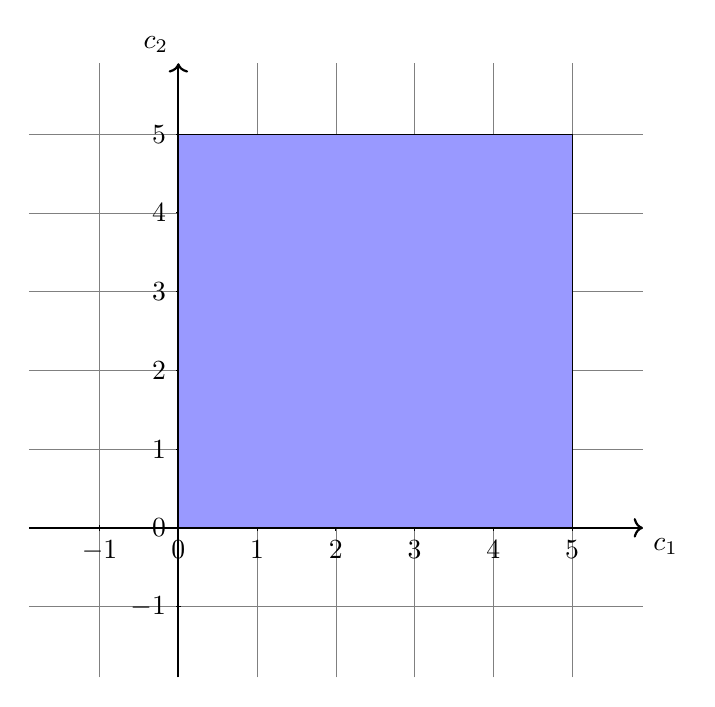
\begin{tikzpicture}

\draw[step=1cm,gray,very thin] (-1.9,-1.9) grid (5.9,5.9);

%\shadedraw[inner color=blue,outer color=red, draw=black] (0,0) rectangle (4,4);

\draw[thick,->] (-1.9,0) -- (5.9,0) node[anchor=north west] {$c_1$};
\draw[thick,->] (0,-1.9) -- (0,5.9) node[anchor=south east] {$c_2$};

\foreach \x in {-1,0,1,2,3,4,5}
    \draw (\x cm,1pt) -- (\x cm,-1pt) node[anchor=north] {$\x$};
\foreach \y in {-1,0,1,2,3,4,5}
    \draw (1pt,\y cm) -- (-1pt,\y cm) node[anchor=east] {$\y$};
    
\filldraw[fill=blue!40!white, draw=black] (0,0) rectangle (5,5);
\end{tikzpicture}
\caption{Resulting zone of DDDs in figure \ref{fig:non-canonical}}
\label{fig:non-canonical-zone}
\end{figure}

The $R_LDDD$ is clearly not canonical. We first define a path in a DDD as the bound on all high edges that are traversed in a single walk from the top node to the true node. A path will only have one bound for each variable pair.

\begin{mydef}[Path-reduced DDD~\cite{ddds}]
A path-reduced DDD ($R_PDDD$) is a locally reduced DDD where all paths are feasible.
\end{mydef}

This definition ensures that all paths in a DDD actually represent a zone, and that there are no redundant paths in the DDD that just represent an empty set. This usage of paths is compatible to the state vectors used in \ltsmin{}. An $R_PDDD$ is still not canonical. We need to define tightness, saturation and disjunctive vertices. To define tightness we first need to define dominating constraints.

\begin{mydef}[Dominating constraint~\cite{ddds}]
A constraint $x_i - x_j \lesssim c$ is dominating in a path $p$ if all other constraints $x_i - x_j \lesssim' c'$ on the same pair of variables in $p$ are less restrictive.
\end{mydef}

\begin{mydef}[Tightness~\cite{ddds}]
A dominating constraint $\alpha = x_i - x_j \lesssim c$ is tight in a feasible path $[p] = [p_1] \wedge \alpha \wedge [p_2]$ if for all tighter constraints $(c', \lesssim') < (c,\lesssim),$ the systems $[p_1] \wedge (x_i - x_j \lesssim' c') \wedge [p_2]$ and $[p]$ have different solutions. A path $p$ is tight if it is feasible and all dominating constraints on it are tight. An $R_LDDD u$ is tight if all paths from $u$ are tight. 
\end{mydef}

\begin{mydef}[Saturation~\cite{ddds}]
A tight path $p$ from an $R_PDDD$ is saturated if for all constraints $\alpha$ not on $p$, if $\alpha$ is added to $p$ either (1) $\alpha$ is not dominating and tight, or (2) the constraint system $[p_1] \wedge \neg\alpha$ is infeasible when $[p]$ is written $[p] = [p_1] \wedge [p_2]$ with all constraints on $p_1$ smaller than $\alpha$ with respect to $\prec$ and all constraints on $p_2$ larger than $\alpha$. An $R_PDDD$ $u$ is saturated if all paths from $u$ are saturated.
\end{mydef}

\begin{mydef}[Disjunctive vertex~\cite{ddds}]
Let $p$ be a path leading to the vertex $u$ in a DDD, and assume $\alpha = cstr(u), h = high(u),$ and $l = low(u)$. Then $u$ is disjunctive in $p$ if $[p] \wedge (\alpha \rightarrow h,l)$ and $[p] \wedge (h \vee l)$ have the same set of solutions.
\end{mydef}

All of these definitions together lead to the following definition of a fully reduced DDD.
 
\begin{mydef}[Fully reduced DDD~\cite{ddds}]
\label{def:RFDDD}
An $R_pDDD$ u is a fully-reduced DDD ($R_FDDD$) if it is tight, saturated and has no disjunctive vertices.
\end{mydef}

We assume that this fully-reduced DDD is canonical and work from that. It is not ensured that this is actually the case, there is no proof for it.

\begin{myconjecture}[Canonical DDD~\cite{ddds}]
\label{def:Canonical-ddd}
If $u$ and $v$ are $R_FDDDs$ with the same set of solutions then $u = v$.
\end{myconjecture}


DDDs can also be used to represent the discrete variables in automata. This is done by translating the variable into a difference constraint. For example $x_1 = 3$ will be translated into $x_1 - 0 \leq 3 \wedge 0 - x_1 \leq -3$, thus resulting into a DDD with two nodes. We will connect the DDD to an LDD to represent discrete variables to limit the number of nodes.

So far we only found the results of two benchmark tests of DDDs, Milner's scheduler and Fischer's protocol~\cite{Møller200253}. Here the DDD approach has been compared with KRONOS and \uppaal{} which were both slower than the DDD implementation. The results of these benchmarks show no memory usage or number of nodes needed.

\subsection{List Decision Diagram}
The DDD nodes are connected to LDD nodes to represent the discrete variables. We will introduce the LDD structure here. An LDD is used to represent variables with integer values, not only binary values. In contrast to MDDs this is done for one value per node. Resulting in nodes with equal size. We will first define the LDD structure.

\begin{mydef}[List Decision Diagram]
\label{def:LDD}
A List Decision Diagram (LDD) is a directed acyclic graph $(V,E)$. The vertex set $V$ contains two terminals $0$ and $1$ with out-degree zero, and a set of non-terminal vertices with out-degree two and the following attributes.
\\\\
\begin{tabular}{lll}
Attribute                & Type                      & Description                                           \\\hline
var(v)                   & \textbf{Var}              & Variable x \\

const(v)                 & $\mathbb{Z}$              & Constant c.                                           \\
high(v), low(v)          & $V$                       & High-branch h, and low-branch l.                   
\end{tabular}
\captionof*{table}{}  
The set E contains the edges $(v,low(v))$ and $(v, high(v))$, where $v \in V$ is a non-terminal vertex.
\end{mydef} 

The definition is almost equal to DDDs, definition \ref{def:DDD}. The difference is the operator that is not in LDDs. LDDs can be seen as a DDD with not a $<$ or $\leq$ as operator, but a $=$. 


\clearpage
\section{Plan}
We will implement first a method that will use the best of both worlds, the efficient algorithms from de DBMs and the memory efficiency of a symbolic approach. We will use the DBMs in the state exploration such that we can find a canonical representation of the clock zone of a newly explored state quite easily. For the symbolic representation of the state space, including the clock zones, and the transition relations, we will use normal BDDs. The DBMs will be flattened and put directly into the state vector and can then be handled by the symbolic BDD back-end. Therefore both the efficient algorithms and the memory efficient representation can be used. A downside to this approach is that a zone subsumption check is not possible anymore, as only equalities and no inequalities can be checked on BDDs, resulting in revisiting of some states. Further we will focus on efficient orderings of the BDDs, as both clock zones and states are contained in a single structure. We will also use this new method with the existing multi-core tool, such that we can still use the subsumption check that is implemented in \ltsmin{}. Afther that we will continue towards a DDD model checker. First we will use the DDDs as the state space representation and still use the language module using the DBMs. We have not been able to find any literature on the combination of these techniques. There might be a significant memory improvement possible here. Eventually we aim at a complete symbolic solution with more operations on the DDD, such as the progress of time, then we can have a language module which does not use the DBMs any more. We will compare the different approaches we implement extensively to each other. All of these approaches will be implemented in the \ltsmin{} toolset. This way we can really compare the methods and not just the tools.

Alongside this we will also have to make the Opaal \pins{} work with the \uppaal{} models generated by ANIMO. The current versions doe not work together because of global variables are used in the system declaration in the generated model, and this is a feature that Opaal does not support. We can make this work by either changing the models generated by ANIMO or by extending the Opaal \pins{}. At this time we do not know the best solution for this problem.


\subsection{Questions}
For the research we will state a couple of research questions:
{\renewcommand\labelitemi{--}
	\begin{itemize}
		\item Is the combination of BDDs and flattened DBMs an efficient method for symbolic reachability analysis of timed automata? Both on memory usage and speed.
		\item Can improvements be achieved by using different orderings? Both by changing the order of only the clock variables and by mixing the clock and state variables.
		\item Is the new language module needed for the symbolic approach also usable for the multi-core approach with subsumption?
		\item Can the BDD approach be generalized towards a method using DDDs?
		\item Is a fully symbolic reachability analysis using DDDs more efficient than the combination of DDDs and DBMs, both on memory and speed?
	\end{itemize}
}

\subsection{Algorithms}
To create a DDD library we will implement a number of functions over DDDs. We will limit the functions to the ones needed for this purpose. Therefore it will not become a complete DDD package. One of the core operations on DDDs is the apply operation. This operation takes two DDDs and a binary operator and combines the two DDDs according to the operator. The apply function for DDDs is a generalisation of the function for BDDs. In ~\cite{ddds} a general definition of the algorithm is given. We turned this more mathematical definition into an algorithm, we give pseudo-code in Algorithm \ref{alg:apply}. In Algorithm \ref{alg:union} we give the pseudo-code for the apply function with the or operator, or the union function, this way we can increase performance by not going down the entire diagram if we already found a terminal. All functions rely on a Mk function which checks if the node needed already exists, and otherwise creates a new node.
The subsumption check, which we lost in the BDD approach, will be possible again with DDDs. This will be the same check as a state membership in an LDD. The only difference is that no equality, but upper bounds will be checked. Pseudo-code for this algorithm is given in Algorithm \ref{alg:contain}. If we combine DDDs with LDDs, only the correct check has to be adapted, checking for equalities, not inequalities, the algorithm will remain the same.

\begin{comment}
In BDDs it is simple to test for containment of a state. This can be done in linear time over the number of variables. For zones in DDDs this can be a harder question, as a zone can be contained in some larger zone in the DDD. For this we need an extension to the normal LDD algorithm, that can handle these zones. The main difference is that on some nodes both the high and the low edge can lead to a satisfying path. Algorithm \ref{alg:containOLD} tests if a zone $z$ is contained in the DDD rooted at $v$.

\begin{algorithm}
\caption{Zone containment for DDDs}\label{alg:containOLD}
\begin{algorithmic}[1]
\Procedure{Contains}{$v, z$}
	\If{$v \in {0,1}$} 
		\Return{$v$} 
	\EndIf
	\If{z[$var(v)$] correct in $v$}
		\If{\Call{Contains}{$high(v), z$}} 
			\Return{\True}
		\Else{ 
			\Return{\Call{Contains}{$low(v), z$}}} 
		\EndIf
	\Else{ 
		\Return{\Call{Contains}{$low(v), z$}}} 
	\EndIf
\EndProcedure
\end{algorithmic}
\end{algorithm}

Where the correct in check will evaluate if the upper-bound in the zone is lower than the upper bound in the node $v$. As we will use maximal sharing of subtrees, some nodes might be revisited. Once we revisit a node, we know that none of it subtrees will lead to a correct evaluation. Therefore we could use a visited flag, to save computation time. The worst case running time of the algorithm will be $\mathcal{O}(|v|)$, where $|v|$ is the number of nodes in the DDD. This can increase the running time of the state space generation significantly, as this algorithm will need to be ran every time a new state is found. It will however save memory, as no zones will be added that are already in the DDD. As the main goal of a symbolic approach is the reduction of memory, we think this is the better solution, over a less time consuming approach which would lead to more memory consumption. The algorithm will not work correctly when the discrete variables are also translated into DDD nodes, as the value in those cases needs to be correct, and an higher upper bound will not work. For the mix of DDD and LDD nodes we will need to change the algorithm to algorithm \ref{alg:containLDD}. This algorithm checks if a node is of type DDD. If it is, the old algorithm will be executed normally, if not, then it is an LDD node and in case of a correct evaluation only the high edge will be explored. The low edge will in that case never lead to a correct evaluation of the state.

\begin{algorithm}
\begin{algorithmic}[1]
\caption{Zone containment for mixed diagram}\label{alg:containLDD}
\Procedure{Contains}{$v, z$}
	\If{$v \in {0,1}$} 
		\Return{$v$} 
	\EndIf
	\If{z[$var(v)$] correct in $v$}
		\If{$type(v)$ is DDD} 
			\If{\Call{Contains}{$high(v), z$}} 
				\Return{\True}
			\Else{ 
				\Return{\Call{Contains}{$low(v), z$}}} 
			\EndIf
		\Else{
			\Return{\Call{Contains}{$high(v), z$}}}
		\EndIf 
	\Else{ 
		\Return{\Call{Contains}{$low(v), z$}}} 
	\EndIf
\EndProcedure
\end{algorithmic}
\end{algorithm}

\end{comment}

\begin{algorithm}
\begin{algorithmic}[1]
\caption{Apply}\label{alg:apply}
\Procedure{Apply}{$v1, v2, op$}
	\If{$v1 \in \{0,1\} \wedge v2 \in \{0,1\}$}
		\State $result \gets (v1$ $op$ $v2)$
	\ElsIf{$var(v1) \prec var(v2)$}
		\State $high \gets$ \Call{Apply}{$high(v1), v2, op$}
		\State $low \gets$ \Call{Apply}{$low(v1), v2, op$}
		\State $result \gets$ \Call{Mk}{$cstr(v1), high, low$} 
	\ElsIf{$var(v2) \prec var(v1)$}
		\State $high \gets$ \Call{Apply}{$high(v2), v1, op$}
		\State $low \gets$ \Call{Apply}{$low(v2), v1, op$}
		\State $result \gets$ \Call{Mk}{$cstr(v2), high, low$} 
	\ElsIf{$v1 \prec v2$}
		\State $high \gets$ \Call{Apply}{$high(v1), high(v2), op$}
		\State $low \gets$ \Call{Apply}{$low(v1), v2, op$}
		\State $result \gets$ \Call{Mk}{$cstr(v1), high, low$}
	\ElsIf{$v2 \prec v1$}
		\State $high \gets$ \Call{Apply}{$high(v1), high(v2), op$}
		\State $low \gets$ \Call{Apply}{$v1, low(v2), op$}
		\State $result \gets$ \Call{Mk}{$cstr(v2), high, low$}
	\ElsIf{$v1 = v2$}
		\State $high(v1) \gets$ \Call{Apply}{$high(v1), high(v2), op$}
		\State $low(v1) \gets$ \Call{Apply}{$low(v1), low(v2), op$}
		\State $result \gets$ \Call{Mk}{$cstr(v1), high, low$}
	\EndIf
	\State \Return $result$
\EndProcedure
\end{algorithmic}
\end{algorithm}

\begin{algorithm}
\begin{algorithmic}[1]
\caption{Union}\label{alg:union}
\Procedure{Union}{$v1, v2$}
	\If{$v1 = v2$} 
		\Return{$v1$} 
	\ElsIf{$v1 =$ \False}
		\Return{$v2$}
	\ElsIf{$v2 =$ \False}
		\Return{$v1$}
	\ElsIf{$var(v1) \prec var(v2)$}
		\State $high \gets$ \Call{Union}{$high(v1), v2$}
		\State $low \gets$ \Call{Union}{$low(v1), v2$}
		\State $result \gets$ \Call{Mk}{$cstr(v1), high, low$} 
	\ElsIf{$var(v2) \prec var(v1)$}
		\State $high \gets$ \Call{Union}{$high(v2), v1$}
		\State $low \gets$ \Call{Union}{$low(v2), v1$}
		\State $result \gets$ \Call{Mk}{$cstr(v2), high, low$} 
	\ElsIf{$v1 \prec v2$}
		\State $high \gets$ \Call{Union}{$high(v1), high(v2)$}
		\State $low \gets$ \Call{Union}{$low(v1), v2$}
		\State $result \gets$ \Call{Mk}{$cstr(v1), high, low$}
	\ElsIf{$v2 \prec v1$}
		\State $high \gets$ \Call{Union}{$high(v1), high(v2)$}
		\State $low \gets$ \Call{Union}{$v1, low(v2)$}
		\State $result \gets$ \Call{Mk}{$cstr(v2), high, low$}
	\ElsIf{$v1 = v2$}
		\State $high(v1) \gets$ \Call{Union}{$high(v1), high(v2)$}
		\State $low(v1) \gets$ \Call{Union}{$low(v1), low(v2)$}
		\State $result \gets$ \Call{Mk}{$cstr(v1), high, low$}
	\EndIf
	\State \Return $result$
\EndProcedure
\end{algorithmic}
\end{algorithm}

\begin{algorithm}
\caption{Zone containment for DDDs}\label{alg:contain}
\begin{algorithmic}[1]
\Procedure{Contains}{$v, z$}
	\If{$v \in {0,1}$} 
		\Return{$v$} 
	\ElsIf{z[$var(v)$] correct in $v$}
		\State\Return{\Call{Contains}{$high(v), z$}} 
	\Else{ 
		\Return{\Call{Contains}{$low(v), z$}}} 
	\EndIf
\EndProcedure
\end{algorithmic}
\end{algorithm}

\subsection{Planning}
In this section we describe all things that need to be implemented to make model checking with a certain diagram possible. 

To make symbolic model checking work we need to change the Opaal \pins{}. The \pins{} currently uses a pointer to a DBM. For the new approach we will put the values of the DBM directly into the state vector. This will increase the size of the state vector. All other references to the types and values of the state vector entries will need to be changed also. (1)

To make symbolic variable reordering possible we will need to partition the next-state function. In the code the next-state function is already split up per transition, but in a single transition group. Splitting this into multiple transition groups should not be too hard. (2)

Once the next-state function is partitioned, also a sparse dependency matrix is needed. This will need to be created according to the transition groups. After this step the variable reordering steps in \ltsmin{} need to work. (3)

To combine the new \pins{} with the multi-core \ltsmin{} back-end the subsumption check will need to be changed. This check now relies on a pointer to a DBM, but it will now get the complete DBM, or state vector. Here the search algorithm or the subsumption check will need to know which variables are zone variables. It will also occur that different states will have the same discrete variables, but different zone variables, these all need to be checked for the subsumption check. (4)

For the combination with the multi-core back-end also the data structure will need to be adapted. The current structure stores a discrete state together with a set of pointers to DBMs. In the new situation each pair of discrete state and DBM will be stored explicitly. (5)

To use a DDD approach, the first step will be to create a minimal DDD library that has the functionality to save a state space. This library will probably miss some features for more advanced model checking techniques. (6)

Once we have a DDD library, we need to combine this with nodes to represent discrete state variables. The main candidate for this are LDD nodes, as they share the same structure with DDDs. (7)

For the combination of DDD and LDD nodes, the diagram will need to be able to identify the zone variables from the discrete state variables in the state vector. This will need an extra function in the \pins{} interface recognizing the different types of variables. (8)

For the DDD representation the values from the DBM will need to be translated to useful variables as ordering of the DDD is based on the values. Also to check for inequalities and set containment the meaningful values are needed. In the current DBM library both the value and the operator are saved in a single 32 bit integer. The DDD will need to know the value and the operator separately.
In this section we describe all things that need to be implemented to make model checking with a certain diagram possible. (9)

Once we have a working DDD representation the first set of benchmark tests can be conducted. This will be the big set of tests for the BDD, DDD and multi-core approach, we can compare these to the old multi-core approach and to the newest version of \uppaal{}. (10)

To continue towards a fully symbolic approach, we will need to extend the DDD libary with some functions. We need for example a function to let time progress, and to set invariants over the states. (11)

For the fully symbolic approach again the language module will need to be adapted. We will no longer need the DBM in the language module. The module will only need to change the discrete state variables, the zone variables will be adapted in the diagram. (12)

If we have this fully symbolic approach this will also need to be tested. We will conduct the same tests as we did for the other approaches, such that we can compare this diagram to all earlier approaches. (13)

In the table below we have put all actions that need to be done into tasks. In the second column we put which tool should work correctly for the Opaal language module after the task. This will give us intermediate points on which we can test the work that has been done to that point.

\begin{center}
%\begin{table}[]
%\centering
%\caption{My caption}
%\label{my-label}
\begin{tabular}{@{}lll@{}}
\toprule
Task                                           & Needs to function                                                           & Date       \\ \midrule
Start                                          &                                                                             & 01-02-2016 \\
Flatten the DBMs (1)                           & Symbolic tool                                                               & 15-02-2016 \\
Partition the next-state function (2)          & Symbolic tool                                                               & 01-03-2016 \\
Create dependency matrices (3)                 & \begin{tabular}[c]{@{}l@{}}Symbolic tool\\ variable reordering\end{tabular} & 15-03-2016 \\
Subsumption check for multi-core back end (4)   &                                                                             & 01-04-2016 \\
Other adaptions multi-core approach (5)         & Multi-core tool                                                              & 01-04-2016 \\
Create minimal DDD library (6)                 &                                                                             & 15-04-2016 \\
Combine DDD with LDD (7)                       &                                                                             & 01-04-2016 \\
Language module for DDD approach (8, 9)        & Symbolic tool                                                               & 08-04-2016 \\
Benchmark tests for multiple approaches (10)   &                                                                             & 15-04-2016 \\
Test with ANIMO models                         &                                                                             & 15-04-2016 \\
DDD library for fully symbolic approach (11)   &                                                                             & 15-05-2016 \\
Language module for fully symbolic DDDs (12)   & Symbolic tool                                                               & 01-06-2016 \\
Benchmark Testing fully symbolic approach (13) &                                                                             & 15-06-2016 \\
Writing Report                                 &                                                                             & 01-07-2016 \\ \bottomrule
\end{tabular}
\end{center}

%\end{table}

\clearpage
\section{Notes}
\subsection{Successor Generator}
The language module uses the opaal successor generator for \uppaal{} models. This generator is written in Python and reads \uppaal{} XML files. A C++ file is generated from this. These files are compiled to object files which can be dynamically linked to \ltsmin{}. The structure of the next-state function is slightly different from ~\cite{eemcs21972}. The new structure can be found in algorithm \ref{alg:successor-gen}. Al line \ref{lst:line:alltrans}, the function iterates over all outgoing transitions from the current location. If it is an internal transition the successor will be generated on lines \ref{lst:line:normaltrans}-\ref{lst:line:endnormaltrans}. If it is a sending transition, receivers will be searched for on lines \ref{lst:line:synctrans}-\ref{lst:line:endsynctrans}. In the generated C++ code the loops on lines \ref{lst:line:alllocs} and \ref{lst:line:alllocs2} are unrolled. The algorithm contains several empty checks, on lines \ref{lst:line:empty1},  \ref{lst:line:empty2}, \ref{lst:line:empty3} and \ref{lst:line:empty4}. After each addition of constraints the DBM can possibly be empty. If the DBM is at one of these points empty, no point in time exists where the new state can exist, so further exploration of the transition is not needed. After the empty checks on lines \ref{lst:line:empty2} and \ref{lst:line:empty4} the extrapolation and the reduction are done. These operations can not empty the DBM, the extrapolation can make the zone larger, not smaller. The reduction will not change the zone at all, only its representation. If the DBM is not empty before these operations it can safely be put into the output.

\begin{algorithm}
\caption{Next-State}\label{alg:successor-gen}
\begin{algorithmic}[1]
\Procedure{Next-State}{$s_{in} = \{l_1,...l_n,l_{n+1},...,l_m\}$}
	\State $out\_states := \emptyset$	
	\State $D := $\Call{CreateDBM}{$\{l_{n+1},...,l_m\}$}		
	\State \Call{TightenDBM}{$D$}
	\For{$l_i \in l_1,...,l_n$} \label{lst:line:alllocs}
		\ForAll{$l_i \xrightarrow{g,a,r} l_i'$} \label{lst:line:alltrans}
			\State $D' := D \cap g$
			\If{$D' \neq \emptyset$}\label{lst:line:empty1}
				\If{$a = \tau$} \label{lst:line:normaltrans}
					\State $D' := D'[r]$
					\State $D' := D'\uparrow$
					\State $D' := D' \cap I_C^i(l_i') \cap \bigcap_{k \neq i} I_C^k(l_k)$
					\If{$D' \neq \emptyset$}\label{lst:line:empty2}
						\State $D' := D'/ B(l_1,...,l_i',...,l_n)$
						\State \Call{ReduceZero}{$D'$}
						\State $\{l_{n+1}',...,l_m'\} := $\Call{FlattenDBM}{$D'$}
						\State $s_{out} := \{l_1,...,l_i',...,l_n,l_{n+1}',...,l_m'\}$
						\State $out\_states := out\_states \cup s_{out}$
					\EndIf \label{lst:line:endnormaltrans}
				\Else
					\If{$a = ch!$} \label{lst:line:synctrans}
						\For{$l_j \in l_1,...,l_n, j \neq i$}\label{lst:line:alllocs2}
							\ForAll{$l_j \xrightarrow{g_j,ch?,r_j} l_j'$}
								\If{$D'' "= D' \cap g_j \neq \emptyset$}\label{lst:line:empty3}
									\State $D'' := D''[r][r_j]$
									\State $D'' := D''\uparrow$
									\State $D'' := D'' \cap I_C^i(l_i') \cap I_C^j(l_j') \cap \bigcap_{k \neq \{i,j\}} I_C^k(l_k)$
									\If{$D'' \neq \emptyset$}\label{lst:line:empty4}
										\State $D''	:= D''/ B(l_1,...,l_i',...,l_j',...,l_n)$						
										\State \Call{ReduceZero}{$D''$}		
										\State $\{l_{n+1}',...,l_m'\} := $\Call{FlattenDBM}{$D'$}
										\State $s_{out} := \{l_1,...,l_i',...,l_j',...,l_n,l_{n+1}',...,l_m'\}$
										\State $out\_states := out\_states \cup s_{out}$
									\EndIf								
								\EndIf							
							\EndFor
						\EndFor \label{lst:line:endsynctrans}
					\EndIf
				\EndIf
			\EndIf
		\EndFor
	\EndFor
	\State \Return $out\_states$
\EndProcedure
\end{algorithmic}
\end{algorithm}

\subsection{Time Extrapolation}
\label{subsec:extrapolation}
In the successor generator step a time extrapolation is used. This extrapolation step reduces the number of DBMs created and makes sure that this number is finite. The most coarse abstraction as described in ~\cite{Behrmann2004} is used. This extrapolation reduces the number of zones that are explored significantly. It also makes that less improvements can be made on the representation of the zones, for some models all states are extrapolated to the same zone, so nothing interesting happens at the timed side of the model any more. In opaal this algorithm is implemented in such a way that all \uppaal{} locations are always read. The maximum extrapolation is based on the values of these locations. Only if there is no difference between all values for a certain location, it is not needed to read this. This results into an densely populated dependency matrix. 

\subsection{Animo Models}
We started the project with ANIMO models that were not compatible with opaal. As opaal does only support a subset of all options of \uppaal{}. First of all we changed the model, such that it does not use global variables in in the system declaration. Also some smaller changes to the use of structs had to be made. This resulted in a basic ANIMO model that is compatible. Larger models are still not compatible due to clock guards on input synchronization channels. This is a feature only recently implemented by \uppaal{}(version 4.1.3). Opaal does not support this feature, and its semantics are not completely clear, as it is not described in the manual. Adding this to opaal can be done, but is not trivial. This improvement of the language module is out of scope of this thesis.  

\subsection{Correctness}
The DDD state space generator needs to be checked for correctness to say anything about the results. We only checked for partial correctness by comparing discrete states. Counting the discrete state-space can be done by counting the number of paths until the first DDD level in the diagram. These numbers were compared to the discrete state space in the LDD solution without reordering, here the discrete state-space can also be determined by counting paths until the first level representing zones. We can not directly compare state-spaces to \uppaal{}, different representations of the timing part of the state-space can give different numbers.


\clearpage
\section{Time Extrapolation}
In the successor generator step a time extrapolation is used. This extrapolation step reduces the number of DBMs created and makes sure that this number is finite. The most coarse abstraction as described in ~\cite{Behrmann2004} is used. This extrapolation reduces the number of zones that are explored significantly. It also makes that less improvements can be made on the representation of the zones, for some models all states are extrapolated to the same zone, so nothing interesting happens at the timed side of the model any more. In opaal this algorithm is implemented in such a way that all \uppaal{} locations are always read. The maximum extrapolation is based on the values of these locations. Only if there is no difference between all values for a certain location, it is not needed to read this. This results into an densely populated dependency matrix. 

\clearpage
\section{Benchmarks}
Below we describe the different models we used to run the benchmarks. We tried to find models that scale up for a number of nodes or processes, so that we can also check the behaviour of our approaches for different sizes of the same model. We summarized the number of nodes and clocks in Table \ref{tab:experiments-variables}

\subsection{Viking}
The set of Viking tests, models the classical Viking and bridge problem. It models 4 Vikings at a dark bridge, they only carry one torch. The torch is only strong enough to give light for 2 Vikings. All Vikings have different walking speeds, a faster Viking will have to adapt to a slower one, when crossing the bridge together. The walking speed of the Vikings is modelled by time constraints on the action of letting go of the torch. The model has a low number of discrete variables, one per Viking, one for the torch and an indicator for the side of the bridge on which the torch is. It has a global clock and a clock per Viking. The standard version of this problem has 4 Vikings. This can however be generalized to $n$ Vikings.

The model results in a densely filled dependency matrix. The torch and all Viking variables are always read for the time extrapolation. Only the side indicator is not always read. The write matrix is sparser. 

The difference between the LDD representation with flattened DBMs and the DDD representation is quite small for this model. In the extrapolation step all clock zones are set to $[0..\infty]$ for all states, so in both diagrams the zones are represented by a single path. So the interesting things are only happening in the discrete parts.

\subsection{Fischer}
Fischer's mutual exclusion protocol~\cite{Lamport:1987:FME:7351.7352} is modelled for a number of processes. There is no synchronization between processes, only blocking of actions can occur. This model has a slightly higher number of discrete variables compared to the Viking tests. Each process has a location and an id. The model also has 2 global discrete variables. Each process has a local clock, no global clock is used.

The dependency matrix of this model has some sparse rows, as each model has an id, which is a constant and can only be read. Again, all the location variables are always read due to the time extrapolation. 

\subsection{CSMA-CD}
The Carrier Sense Multiple Access/Collision Detection~\cite{kronos} is modelled for a number of senders. The model has a few discrete variables, it only has locations and one global counter. The system is modelled with a single bus and $n$ senders. Each sender and the bus have a local clock, no global clock is used. The model uses a lot of synchronizations between the senders and the bus.

\subsection{Animo}
We could not use the ANIMO models, only the smallest model with no synchronizations was possible. As we started the project to work on ANIMO models, we still included that single model in the benchmark set. It is a model with only one node, so only one location variable. The model has two clocks, a global clock and a clock for the node.  Further it does have quite a large number of discrete variables. Both the global declaration and the node have a portion of C-like code with a number of global variables. 

This results in a model with a quite sparse dependency matrix, as only the single location is used for the time extrapolation. We expected this model to have good performance for the LDD method with variable reordering.

\subsection{Lynch-Shavit}
The Lynch-Shavit mutual exclusion protcol~\cite{LS} is modelled for different number of processes. The structure of the model is quite like the Fischer model. It only uses one global variable more than Fischer.

\subsection{Milner}
Milners scheduler~\cite{Milner:1989:CC:534666} is modelled for a number of nodes. The structure is like that of the CSMA-CD model, except that it does not use a bus. The model has a lot of synchronizations between the nodes, and between the node and a global process. Each node has two clocks, so the zone representation blows up quickly. 

\subsection{Other models}
We also used some models that we could not scale up enough due to memory/time limitations, or that could not scale up due to the nature of the model. We will not describe those models in detail. These models were the critRegion, Critical, bocdp(-fixed)~\cite{641264}, bando and timelock model.

\begin{table}
\label{tab:experiments-variables}
    \begin{tabular}{|l|l|l|l|l|}
    \hline
     Model  & Parameters  & Components & Clocks & Discrete variables \\ \hline
    Viking  & n vikings   & n + 1      & n + 1  & n + 2              \\
    Fischer & n processes & n          & n      & 2n+2               \\
    CSMA-CD & n stations  & n + 1      & n + 1  & n + 2              \\
    Animo   & n nodes     & n          & n + 1  & 9n + 7             \\
    Lynch   & n processes & n          & n      & 2n + 3             \\
    Milner  & n processes & n + 1      & 2n + 1 & n + 1              \\
    HDDI    & n stations  & n + 1      & 3n + 1 & n + 1              \\ \hline
    \end{tabular}
\caption{Experiment models}
\end{table}

\subsection{Benchmark Runs}
We ran benchmarks with the different solutions we described to compare them to each other. The DDD solution has been ran with the two BFS-prev algorithms as explained in Section \ref{subsection:bfs}; we also used the BFS algorithm from \ltsmin{}. For the LDD solution we only used the original BFS-prev algorithm. We ran this without reordering and with some of the reordering algorithms that \ltsmin{} provides. We used the options gsa, rb4w, cw, rs,rn, rs,ru. These results are compared to the explicit-state multi-core \ltsmin{} and the original \uppaal{}. All experiments have been done with and without the DBM reduction, described in Section \ref{subsection:dbm_reduction}. All solutions are ran with one thread. The LDD and explicit-state multi-core solutions can be ran with multiple threads. The DDD solution does not support this, so for comparison reasons, all methods are used in single-core mode. We also used the new language module with flattened DBMs in combination with the explicit-state multi-core tool.


\clearpage
\section{Results}
In this section we will only give an overview of all experiment results. The complete tables with all results are added in Appendix \ref{app:results}. In Table \ref{tab:time_results} and Table \ref{tab:node_results} we have summarized the results for some of the most interesting models. For the DDD, LDD and mc-flattened column, we give the best result that was found in the different experiment setups. 

\subsection{Time}
The timed results show that our symbolic solutions are slower for almost all models, compared to both \uppaal{} and the explicit state multi-core tool. Only for the small bocdp models we have a symbolic solution that is faster than \uppaal{}. 

One of the reasons we found was the high number of next-state calls. This is much higher than for the explicit-state tool as we partitioned the next-state function. For symbolic solutions this should be an advantage, as locality of transitions can be used. This same advantage should hold for the LDD solution we have, but the dependency matrices are too densely filled to give a real advantage. For the DDD solution we do not even make use of these localities, so there all advantages are lost. To confirm this hypothesis we also ran experiments without the partitioned next-state function. This gave for almost all models much better results. The results differ from a small loss in speed to a speedup of a factor 10. This is still not enough to compete with \uppaal{}, but makes it possible to explore larger models within a given time-bound. 

Another problem seems to be the flattening of the DBM. This is an extra action that has to be executed in each next-state call, compared to the multi-core tool. This flattening is not a really expensive operation, it is only copying values, but it has to be executed a lot of times. For the DDD approach it is also necessary to close each DBM, as the DDD structure does not guarantee this. This is a more expensive operation and will also be executed in each next-state call. We implemented this in the language module, this closing is used for all experiments, so also for the experiments where it is not explicitly needed. This will also explain why the explicit state tool with subsumption is in most cases faster than the explicit state tool with flattened DBMs and without subsumption, even for models where subsumption will not have a real role, like the Viking models.

The last problem we see are the large state-vectors. This is mostly due to the quadratic size of the DBMs. For each of these variables a DDD level is created. As we have shown earlier, in some cases a lot of these levels will not have any impact on the zone represented. We can exploit this a little by setting these nodes to $(\infty,<)$, but the time-expensive function that does this has too much of an impact on the timing results. The diagram could make much more use of this by skipping levels. This is not possible in our implementation as we only implicitly store the level of each node by its depth. 

\begin{table}

    \begin{tabular}{|l|r|r|r|r|r|}
    \hline
                       & \multicolumn{1}{l|}{DDD}   & \multicolumn{1}{l|}{LDD}   & \multicolumn{1}{l|}{mc-flattened} & \multicolumn{1}{l|}{mc-original} & \multicolumn{1}{l|}{uppaal} \\ \hline
    fischer6           & 481.9 & 48.3  & 19.2         & 0.4         & 0.0    \\
    critRegion4        & 56.3  & 39.5  & 24.3         & 0.5         & 0.1    \\
    Critical\_04-25-50 & TO    & TO    & 1.1          & 0.9         & 0.6    \\
    CSMACD\_08         & 1.9   & 7.3   & 6.9          & 0.5         & 0.1    \\
    viking12           & 17.6  & 18.7  & 10.4         & 0.7         & 1.0    \\
    Lynch5-16          & 34.2  & 120.0 & 50.0         & 0.3         & 0.0    \\
    bocdp              & 0.1   & 0.2   & 0.2          & 0.0         & 0.2    \\
    bocdpFIXED         & 0.2   & 0.2   & 0.1          & 0.0         & 0.3    \\
    bando              & 0.2   & 0.2   & 0.1          & 0.0         & 0.3    \\
    Milner-8Nodes-flat & 0.4   & 1.2   & 1.4          & 0.1         & 0.0    \\
    hddi\_input\_10    & TO    & 93.3  & 43.1         & 0.0         & 0.0    \\ \hline
    \end{tabular}
\caption{Time Results (seconds)}
\label{tab:time_results}
\end{table}

\begin{table}

    \begin{tabular}{|l|r|r|}
    \hline
                       & \multicolumn{1}{l|}{DDD}   & \multicolumn{1}{l|}{LDD}    \\ \hline
    fischer6           & 15156 & 85041  \\
    critRegion4        & 55890 & 100006 \\
    Critical\_03-25-50 & 3291  & 17505  \\
    CSMACD\_08         & 36098 & 321001 \\
    viking12           & 342   & 342    \\
    Lynch5-16          & 49430 & 112397 \\
    bocdp              & 487   & 355    \\
    bocdpFIXED         & 488   & 427    \\
    bando              & 488   & 425    \\
    Milner-8Nodes-flat & 11012 & 30883  \\
    hddi\_input\_10    & TO    & 454246 \\ \hline
    \end{tabular}
\caption{Node Results}
\label{tab:node_results}
\end{table}

\begin{table}
\rotatebox{90}{
    \begin{tabular}{|l|l|ll|ll|l|l|l|}
    \hline
     Model      & Discrete states & DDD     & ~     & LDD     & ~     & mc-flattened & mc-original & Uppaal \\
    ~           & ~               & \#nodes & time  & \#nodes & time  & time         & time        & time   \\ \hline
    fischer6    & ~               & 15156   & 481.9 & 85041   & 48.3  & 19.2         & 0.4         & 0.0    \\
    critRegion4 & ~               & 55890   & 46.3  & 100006  & 39.5  & 24.3         & 0.5         & 0.1    \\
    Critical4   & ~               & -       & TO    & -       & TO    & 1.1          & 0.5         & 0.6    \\
    CSMACD8     & ~               & 96098   & 1.9   & 321001  & 7.3   & 6.9          & 0.5         & 0.1    \\
    Viking12    & ~               & 342     & 17.6  & 342     & 18.7  & 10.4         & 0.7         & 1.0    \\
    Lynch5      & ~               & 49430   & 34.2  & 112397  & 120.0 & 50.0         & 0.3         & 0.0    \\
    bocdp       & ~               & 487     & 0.1   & 355     & 0.2   & 0.2          & 0.0         & 0.2    \\
    bocdpFIXED  & ~               & 488     & 0.2   & 427     & 0.2   & 0.1          & 0.0         & 0.3    \\
    bando       & ~               & 488     & 0.2   & 425     & 0.2   & 0.1          & 0.0         & 0.3    \\
    Milner8     & ~               & 11012   & 0.4   & 30887   & 1.2   & 1.4          & 0.1         & 0.0    \\
    hddi10      & ~               & -       & TO    & 454246  & 93.3  & 43.1         & 0.0         & 0.0    \\ \hline
    \end{tabular}
    }
\end{table}

\subsection{Memory}
We have not measured memory usage. A good symbolic solution will use a lot of memory for caching when it is available. Comparing this to other solutions which use less caching will not be representative. We do compare the number of nodes between the different solutions. 

For most models the best DDD solutions uses less nodes than the best LDD solution. This is what we expected as local reductions on clocks can be made. For the smallest models the LDD sometimes gives less nodes for some reorderings. These models have such low number of clocks that no reductions can be made yet. The bocdp and bando models are the largest models which have a lower LDD than DDD representation. These models have quite a high number of discrete variables with a low number of clocks. For most larger models the LDD solution without reordering is smaller than with reordering. This is probably due to the densely filled matrices, so no good reorderings can be created from them.

There is a difference between the number of nodes for the normal BFS and the BFS without minus. This is possible because we do not use a canonical form of DDDs. Most results show a higher number of nodes for the runs with the minus. In Figure \ref{fig:fragmentation} we show an example of how this can happen. We assume all zones in the figures belong to the same set of locations. In Figure \ref{fig:vis_zone} we have the zone that is already visited. Now a new state with the zone in Figure \ref{fig:cur_zone} is discovered. If the minus is not used, successors of this state are directly generated from the set of locations and this zone. If the minus is used the first zone will first be subtracted before successors are generated. The result of the subtraction is shown in Figure \ref{fig:after_minus_zone}. This is not a convex zone, so a DDD with multiple paths is needed. From this state also other successors can be generated, possibly needing more nodes to be represented. If the newly generated states are then unioned with the visited set the result can again have more nodes than the version without minus. The less fractioned zones in the current set can also have implications on the time results, as less work in the next-state function is needed. On the other hand the next-state function can also need extra time, as some states would otherwise have completely been removed from the current set, and no work for that states would need to be done. 

\begin{figure}[h]

\begin{subfigure}[b]{\textwidth}
\centering
\begin{adjustbox}{max totalheight=.3\textheight}
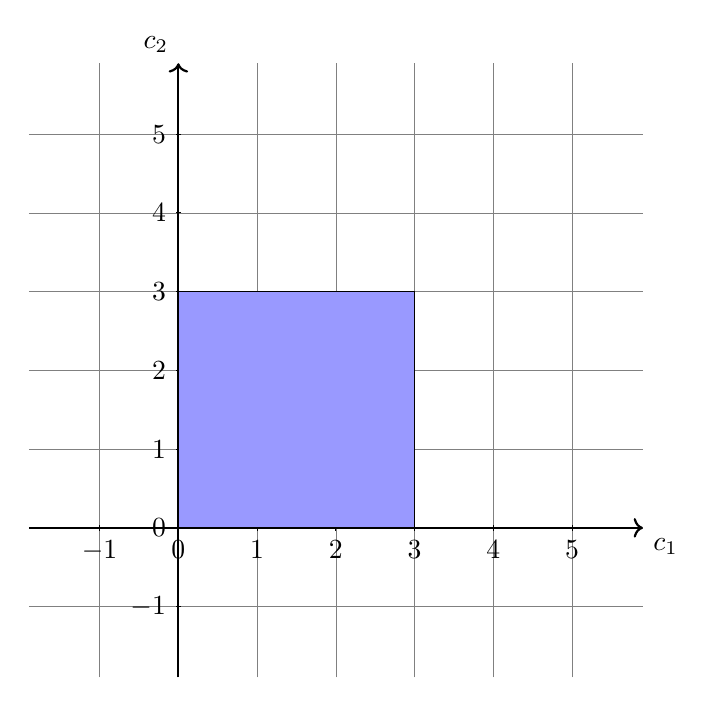
\begin{tikzpicture}

\draw[step=1cm,gray,very thin] (-1.9,-1.9) grid (5.9,5.9);

%\shadedraw[inner color=blue,outer color=red, draw=black] (0,0) rectangle (4,4);

\draw[thick,->] (-1.9,0) -- (5.9,0) node[anchor=north west] {$c_1$};
\draw[thick,->] (0,-1.9) -- (0,5.9) node[anchor=south east] {$c_2$};

\foreach \x in {-1,0,1,2,3,4,5}
    \draw (\x cm,1pt) -- (\x cm,-1pt) node[anchor=north] {$\x$};
\foreach \y in {-1,0,1,2,3,4,5}
    \draw (1pt,\y cm) -- (-1pt,\y cm) node[anchor=east] {$\y$};
    
\filldraw[fill=blue!40!white, draw=black] (0,0) rectangle (3,3);

\end{tikzpicture}
\end{adjustbox}
\caption{Visited Zone}
\label{fig:vis_zone}
\end{subfigure}



\begin{subfigure}[b]{\textwidth}
\centering
\begin{adjustbox}{max totalheight=.3\textheight}
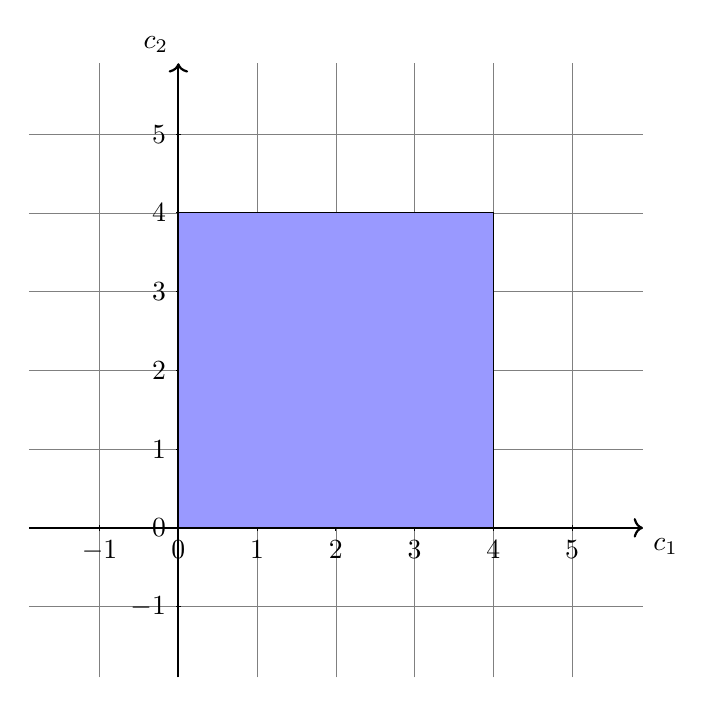
\begin{tikzpicture}
\draw[step=1cm,gray,very thin] (-1.9,-1.9) grid (5.9,5.9);

%\shadedraw[inner color=blue,outer color=red, draw=black] (0,0) rectangle (4,4);

\draw[thick,->] (-1.9,0) -- (5.9,0) node[anchor=north west] {$c_1$};
\draw[thick,->] (0,-1.9) -- (0,5.9) node[anchor=south east] {$c_2$};

\foreach \x in {-1,0,1,2,3,4,5}
    \draw (\x cm,1pt) -- (\x cm,-1pt) node[anchor=north] {$\x$};
\foreach \y in {-1,0,1,2,3,4,5}
    \draw (1pt,\y cm) -- (-1pt,\y cm) node[anchor=east] {$\y$};
    
\filldraw[fill=blue!40!white, draw=black] (0,0) rectangle (4,4);

\end{tikzpicture}
\end{adjustbox}
\caption{Current Zone}
\label{fig:cur_zone}
\end{subfigure}


\begin{subfigure}[b]{\textwidth}
\centering
\begin{adjustbox}{max totalheight=.3\textheight}
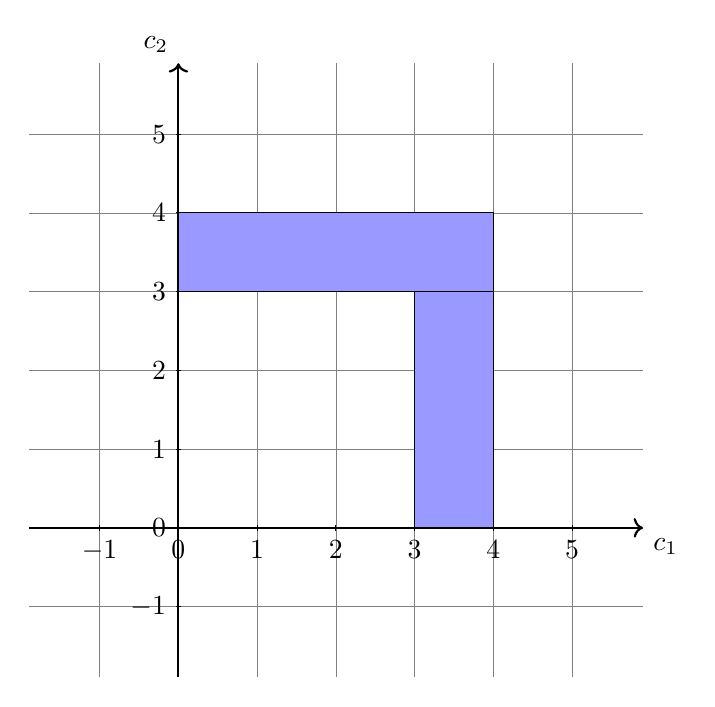
\begin{tikzpicture}
\draw[step=1cm,gray,very thin] (-1.9,-1.9) grid (5.9,5.9);

%\shadedraw[inner color=blue,outer color=red, draw=black] (0,0) rectangle (4,4);

\draw[thick,->] (-1.9,0) -- (5.9,0) node[anchor=north west] {$c_1$};
\draw[thick,->] (0,-1.9) -- (0,5.9) node[anchor=south east] {$c_2$};

\foreach \x in {-1,0,1,2,3,4,5}
    \draw (\x cm,1pt) -- (\x cm,-1pt) node[anchor=north] {$\x$};
\foreach \y in {-1,0,1,2,3,4,5}
    \draw (1pt,\y cm) -- (-1pt,\y cm) node[anchor=east] {$\y$};
    
\filldraw[fill=blue!40!white, draw=black] (0,3) rectangle (4,4);
\filldraw[fill=blue!40!white, draw=black] (3,0) rectangle (4,3);

\end{tikzpicture}
\end{adjustbox}
\caption{After Minus}
\label{fig:after_minus_zone}
\end{subfigure}

\caption{Minus fragmentation}
\label{fig:fragmentation}
\end{figure}

The DBM reduction does not give the results we aimed for. For most models exploration is faster without the reduction. This is due to the expensive algorithm that the reduction is. Also the reduction of the number of nodes is not what we hoped for. Most models get more nodes when the reduction is turned on. The reduction can however still become usefull if we go to a canonical DDD representation. 



\clearpage
\bibliography{references}{}
\bibliographystyle{plain}
\end{document}